\documentclass[a4paper,titlepage]{article}
\usepackage[utf8]{inputenc}
\usepackage{graphicx}
\graphicspath{ {images/} }

\usepackage{url}
\usepackage{siunitx}
\usepackage{natbib}
\usepackage{graphicx}
\usepackage{pgfplots}
\usepackage{indentfirst}
\usepackage{amsmath}
\usepackage{amssymb}
\usepackage{hyperref}
\usepackage{authblk}
\usepackage{multirow}

\pgfplotsset{compat=1.17}
\setlength{\parskip}{1em}

\DeclareMathOperator{\arcsec}{arcsec}
\DeclareMathOperator{\arccot}{arccot}
\DeclareMathOperator{\arccsc}{arccsc}

\title{

\includegraphics[width=4cm]{sst.png}\\
\vspace{1cm}
\textbf{SST Sheltered Walkway}\\
{\large Secondary 3 Additional Mathematics Performance Task}
}

\author{Ryan Theodore The\thanks{ryan\_theodore\_the@s2019.ssts.edu.sg}}
\author{Koh Jieming Xavier\thanks{koh\_jie\_ming\_xavier@s2019.ssts.edu.sg}}
\author{Koh Yi Lei Elliot\thanks{koh\_yi\_lei\_elliot@s2019.ssts.edu.sg}}
\author{Soh Zhi Bing\thanks{soh\_zhi\_bing@s2019.ssts.edu.sg}}
\affil{School of Science and Technology, Singapore}

\date{\today}

\begin{document}

\maketitle

{\setlength{\parskip}{0pt}\tableofcontents}

\pagebreak
\section{Introduction}\label{sec:Introduction}

\subsection{Situation}\label{sec:Introduction:Problem}

In the School of Science and Technology, Singapore (SST), the walkway leading from the school gate to the General Office (GO) is not sheltered. This makes it challenging and inconvenient for students to reach the school building on rainy days. Some of the existing covered walkways in the school may also not be useful in sheltering students during rainy days. 

\subsection{Goals}\label{sec:Introduction:Goals}

\begin{itemize}
    \item Propose a few possible models for the cover of a sheltered walkway in SST in order to solve the current situation.
    \item Prepare a presentation to the school with your analysis and assumptions, mathematical modelling and calculations, and your suggested design with proposed measurements.
\end{itemize}

\begin{figure}[htbp]
    \centering
    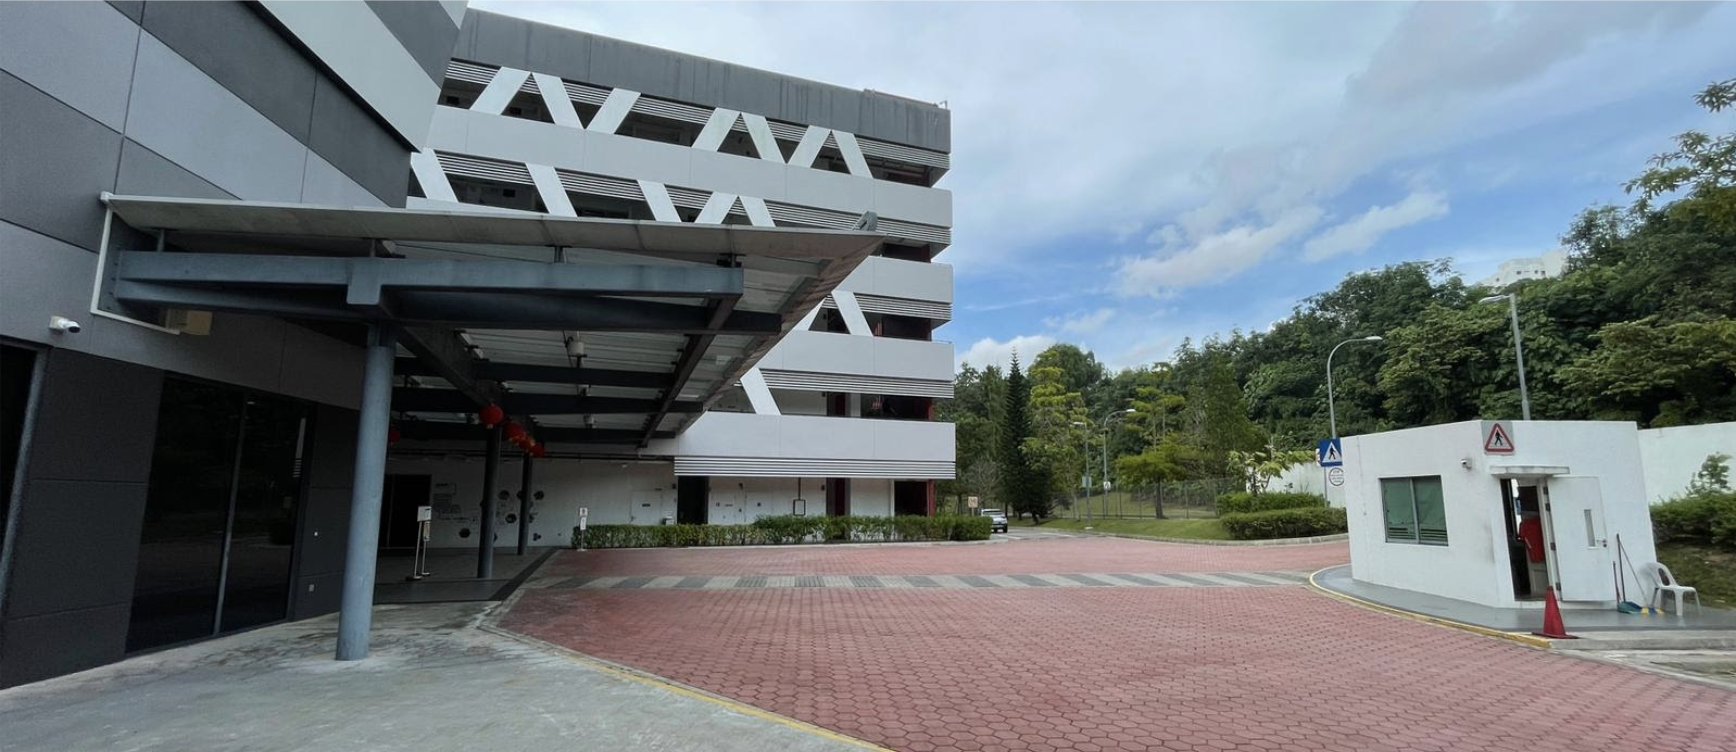
\includegraphics[width=\textwidth]{currentShelter.png}
    \caption{The walkway crossing leading from the school gate to the General Office}
    \label{fig:currentShelter}
\end{figure}

\subsection{Problem Statement}\label{sec:Introduction:Problem Statement}

Students in the School of Science and Technology require a sheltered walkway covering the zebra-crossing from the school's general office to the school gate so that students would be able to leave the school without the need of an umbrella on rainy days, making it more convenient while still ensuring that vehicles are able to use the road.

\subsection{Inspiration}

The designs for this project were inspired by a shelter in Singapore, near Plaza Singapura, which was also displayed in the video provided for this project, like as seen in Figure \ref{fig:downwardsConcaveInspiration}. It is a concaved shelter with a metal frame and a transparent glass/plastic cover.

\begin{figure}[htbp]
    \centering
    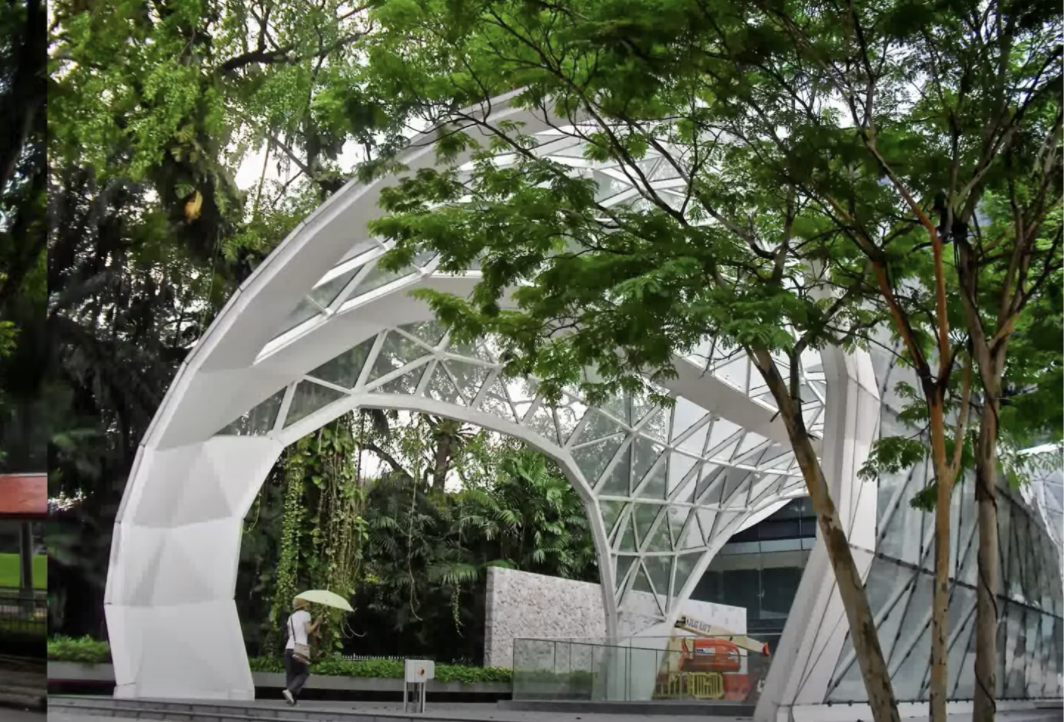
\includegraphics[width=\textwidth]{downwardsConcaveInspiration.png}
    \caption{Inspiration of downwards concave model}
    \label{fig:downwardsConcaveInspiration}
\end{figure}

\pagebreak
\section{Variables}\label{sec:Variables}

\subsection{Controlled Variables}\label{sec:Variables:Controlled Variables}

\subsubsection{Vertical Clearance of Shelter}

The vertical clearance of the shelter refers to the minimum height limit required for our model to succeed, like shown in Figure \ref{fig:verticalClearance}. In Singapore, most vertical clearances are about $4.5\si{m}$ tall, with leeway of about $0.5\si{m}$ at most. It is also an offence to drive a vehicle exceeding $4.5\si{m}$ in height without a police or auxiliary police in Singapore \cite{lta-overheight}. Therefore, it is reasonable to set the vertical clearance of the shelter to be $4.5\si{m}$, with a $0.5\si{m}$ leeway of height, making the total minimum height of our shelter to be $4.5\si{m}+0.5\si{m}=5.0\si{m}$.

\begin{figure}[htbp]
    \centering
    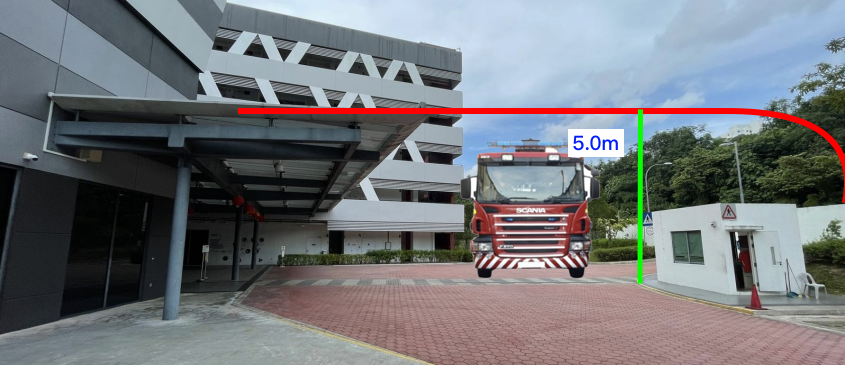
\includegraphics[width=\textwidth]{verticalClearance.png}
    \caption{Required vertical clearance}
    \label{fig:verticalClearance}
\end{figure}

\subsubsection{Horizontal Clearance of Shelter}
\begin{figure}[htbp]
    \centering
    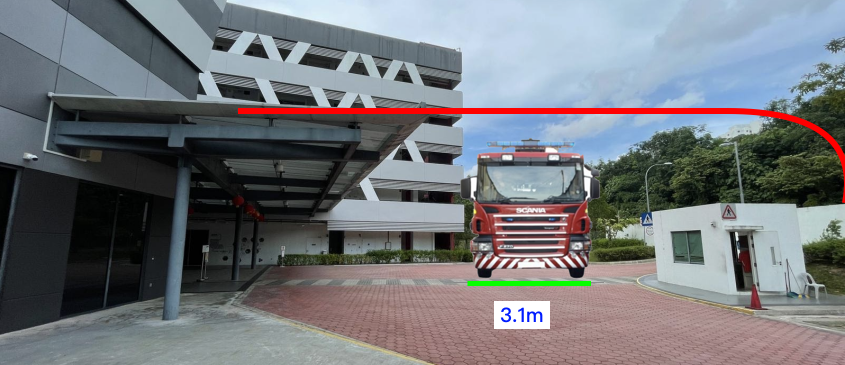
\includegraphics[width=\textwidth]{horizontalClearance.png}
    \caption{Required horizontal clearance}
    \label{fig:horizontalClearance}
\end{figure}
Similar to the vertical clearance, the horizontal clearance of the shelter refers to the minimum width limit required for our model to succeed, like shown in Figure \ref{fig:horizontalClearance}. The standard car lane width in Singapore is about $2.8\si{m}$, but fire trucks may require up to $3.1\si{m}$ in width to pass through\cite{musingsofsgtransport-roadwidth}. Since fire trucks may need to pass under the proposed shelter, it is reasonable to set the horizontal clearance of the shelter to be $3.1\si{m}$.

\subsubsection{Lengths of Walkway Shelter Crossing}
\begin{figure}[htbp]
    \centering
    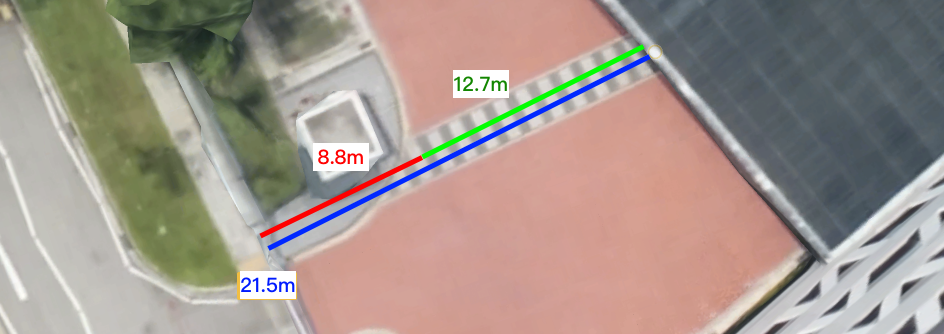
\includegraphics[width=\textwidth]{crossingLength.png}
    \caption{Estimated measurements of length of crossing taken with Google Earth}
    \label{fig:crossingLength}
\end{figure}
The measurements from the school gate of SST to the shelter of the GO, estimated are taken with tools such as Google Earth and Google Street View. The length can be divided into several sections, and the total length, as seen in Figure \ref{fig:crossingLength}:
\begin{itemize}
    \item Distance from Gate to Beginning of Zebra Crossing: $8.8\si{m}$.
    \item Length of Zebra Crossing: $12.7\si{m}$.
    \item Distance from Gate to Shelter: $21.5\si{m}$.
\end{itemize}

\subsubsection{Width of Walkway Shelter Crossing}

As seen in Figure \ref{fig:crossingWidth}, it is estimated that the width of the zebra crossing is about $2.3\si{m}$. Since the shelter should be slightly wider than the zebra crossing, it is sensible for the width of walkway shelter to be $3.0\si{m}$ as seen in Figure \ref{fig:shelterWidth}.

These measurements also fulfill the requirements of minimum $1.5\si{m}$ in width and $2.1\si{m}$ in height, for covered linkways as enforced by the Land Transport Authority, Singapore \cite{lta-coveredlinkedways}.

\begin{figure}[htbp]
    \centering
    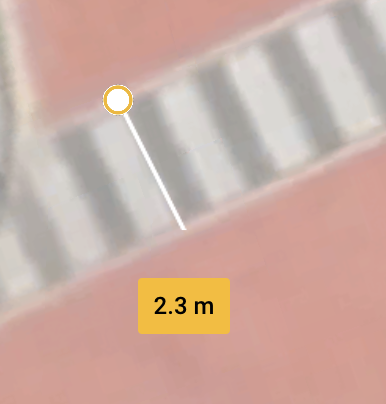
\includegraphics[width=4cm]{crossingWidth.png}
    \caption{Estimated measurement of width of crossing taken with Google Earth}
    \label{fig:crossingWidth}
\end{figure}
\begin{figure}[htbp]
    \centering
    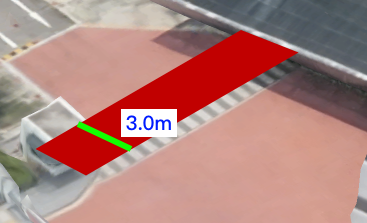
\includegraphics[width=6cm]{shelterWidth.png}
    \caption{Width of the shelter}
    \label{fig:shelterWidth}
\end{figure}

\subsubsection{Height of School Gate}

As seen in Figure \ref{fig:schoolGateHeight}, with the use of Google Earth and Google Street View, it is estimated that the height of the school gate is about $2.5\si{m}$.

\begin{figure}[htbp]
    \centering
    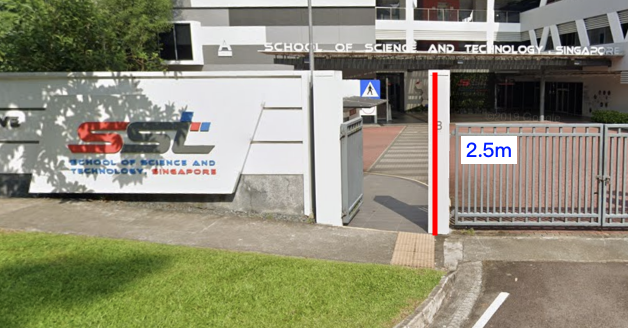
\includegraphics[width=\textwidth]{schoolGateHeight.png}
    \caption{Estimated measurement of height of school gate}
    \label{fig:schoolGateHeight}
\end{figure}

\subsubsection{Height of General Office Shelter}

As seen in Figure \ref{fig:goShelterHeight}, with the use of Google Earth and Google Street View, it is estimated that the height of the shelter above the General Office is about $4.0\si{m}$.

\begin{figure}[htbp]
    \centering
    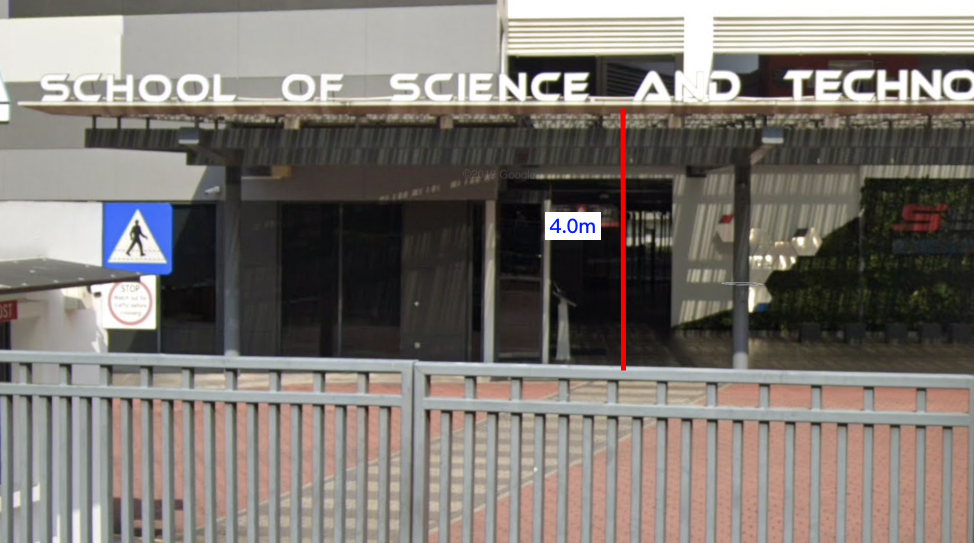
\includegraphics[width=\textwidth]{goShelterHeight.png}
    \caption{Estimated measurement of height of the shelter above general office}
    \label{fig:goShelterHeight}
\end{figure}

\subsubsection{Thickness of Walkway Shelter}
Optimally, the shelter should be as light as possible such that the columns supporting it would not require as much strength to support it. Therefore, a thickness of $1.0\si{cm}$, or $0.01\si{m}$, should suffice, as most shelters are also about this thick.

\subsubsection{Cross-sectional Area of Supporting Columns}
Typical supporting columns are either circular or rectangular but most are less than $20\si{cm}$, or $0.2\si{m}$, in length or diameter.

There are also usually several of these columns which support the weight of the shelter together. For our purposes, it is assumed that 4 of the columns are enough.

According to a research conducted during the California State Science Fair in 2007 \cite{shipp_strengthofshapes}, ``The cylindrical shaped column is the strongest is because of corners. The flat sides of the shapes do not support structural load. Therefore, it is the corners of the shapes that give the columns their strength. The triangle has three corners to support its load, the square has four, the hexagon has six and the octagon has eight corners. In contrast, the circle can be viewed as having 360 corners. Thus, the circle is by far the strongest shaped column.''

Therefore, a cylindrical shaped column that is $0.2\si{m}$ in diameter will be used.

Therefore, a cross sectional area of $0.1\si{m}\cdot0.1\si{m}\cdot\pi\cdot4=0.13\si{m^2}$ (2 SF), for 4 columns at each corner of the shelter, would be reasonable. 

\subsubsection{Mean wind velocity in Singapore}

According to the Meteorological Service Singapore (MSS) which is part of gov.sg \cite{govsg-rainclimate}, ``winds in Singapore are generally light, with the mean surface wind speed normally less than 2.5 m/s''. With this data, the average wind velocity in Singapore can be assumed to be $2.5\si{m/s}$.

\subsection{Independent Variables}\label{sec:Variables:Independent Variables}

\subsubsection{Function of short-side cross-section of shelter}
The short-side cross-section of the shelter refers to the lateral uniform cross-section, with the shortest width, like illustrated in Figure \ref{fig:shortSideFunction}.

\begin{figure}[htbp]
    \centering
    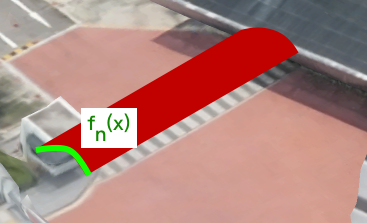
\includegraphics[width=\textwidth]{shortSideFunction.png}
    \caption{Relationship between short-side function and shelter}
    \label{fig:shortSideFunction}
\end{figure}

The short-side cross-section modelled by the functions would determine how water flows off the shelter immediately after it hits the shelter. This would be further investigated in a later section.

\subsubsection{Function of long-side cross-section of shelter}
The long-side cross-section of the shelter refers to the other lateral uniform cross-section, with the longest width, like illustrated in Figure \ref{fig:longSideFunction}.

\begin{figure}[htbp]
    \centering
    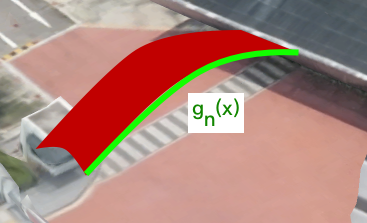
\includegraphics[width=\textwidth]{longSideFunction.png}
    \caption{Relationship between long-side function and shelter}
    \label{fig:longSideFunction}
\end{figure}

The long-side cross-section modelled by the functions would determine how water flows away from the shelter when it rains. This would be further investigated in a later section.

\subsubsection{Material used for shelter}

In order to not put too much strain on the supporting columns holding the shelter up, the material used for the shelter should be as light as possible. This would be further discussed in a later section.

\subsubsection{Material used for columns}

On the other hand, to hold as much weight as possible, the material used for the supporting columns should be as strong as possible to prevent breaking. This would be further discussed in a later section.

\subsection{Dependent Variables}\label{sec:Variables:Dependent Variables}

\subsubsection{Amount of rain likely to get stuck on shelter}

If the shelter is built in a way such that water is able to get trapped on the shelter, this may lead to problems such as mosquito breeding or eventual leakage of the shelter. Therefore, it is crucial to prevent as much water from getting stuck as possible.

There has been an increase in number of dengue cases in recent years. According to the National Environment Agency, Singapore (NEA), between 2019 to 2020, the number of dengue cases in Singapore increased more than twofold, from $663$ to $1792$ cases \cite{nea-dengue}, as seen in Figure \ref{fig:dengueCases}. Hence, it is imperative that the shelter does not allow stagnant water to be trapped, but divert the water away from the shelter.

\begin{figure}[htbp]
    \centering
    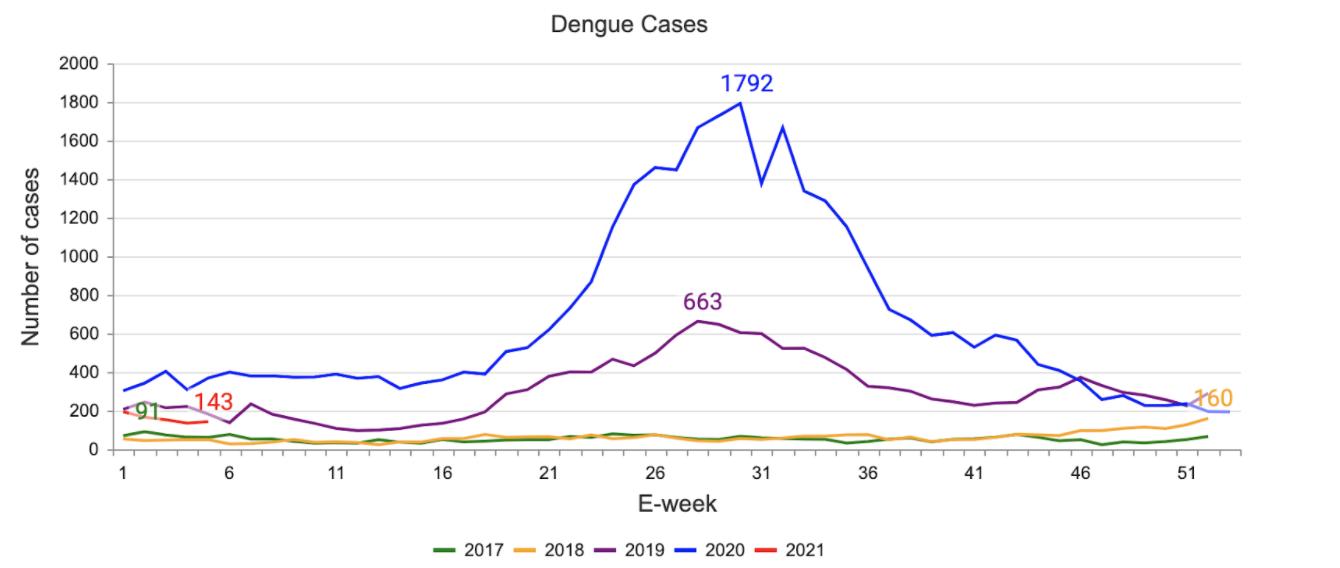
\includegraphics[width=\textwidth]{dengueCases.png}
    \caption{Dengue cases in Singapore over the last few years}
    \label{fig:dengueCases}
\end{figure}

\pagebreak
\subsubsection{Amount of rain likely to hinder pedestrians' vision}

On a stormy and rainy day, it is hard to both drivers and pedestrians to see through the rain. With a shelter overhead displacing all the rain from that area elsewhere, if the rain water collects and falls as thick curtains of water, this would further hinder the sight of people which may lead to road accidents. Therefore, it is important to ensure that the rainwater will not hinder pedestrians' vision.

\subsubsection{Possibility of columns breaking to stress caused by weight}
The support columns will have to be strong enough to withstand the weight of the shelter for a prolonged period of time to prevent the shelter from falling and causing injury or death to students and teachers.

\section{Assumptions and Simplifications}\label{sec:Assumptions and Simplifications}

\subsection{Assumptions}\label{sec:Assumptions and Simplifications:Assumptions}

\subsubsection{Unsheltered walkways of concern}
The unsheltered pathway outside of SST as seen in Figure \ref{fig:unshelteredAreaOutsideSst} does not concern this project as it is not managed by SST.

\begin{figure}[htbp]
    \centering
    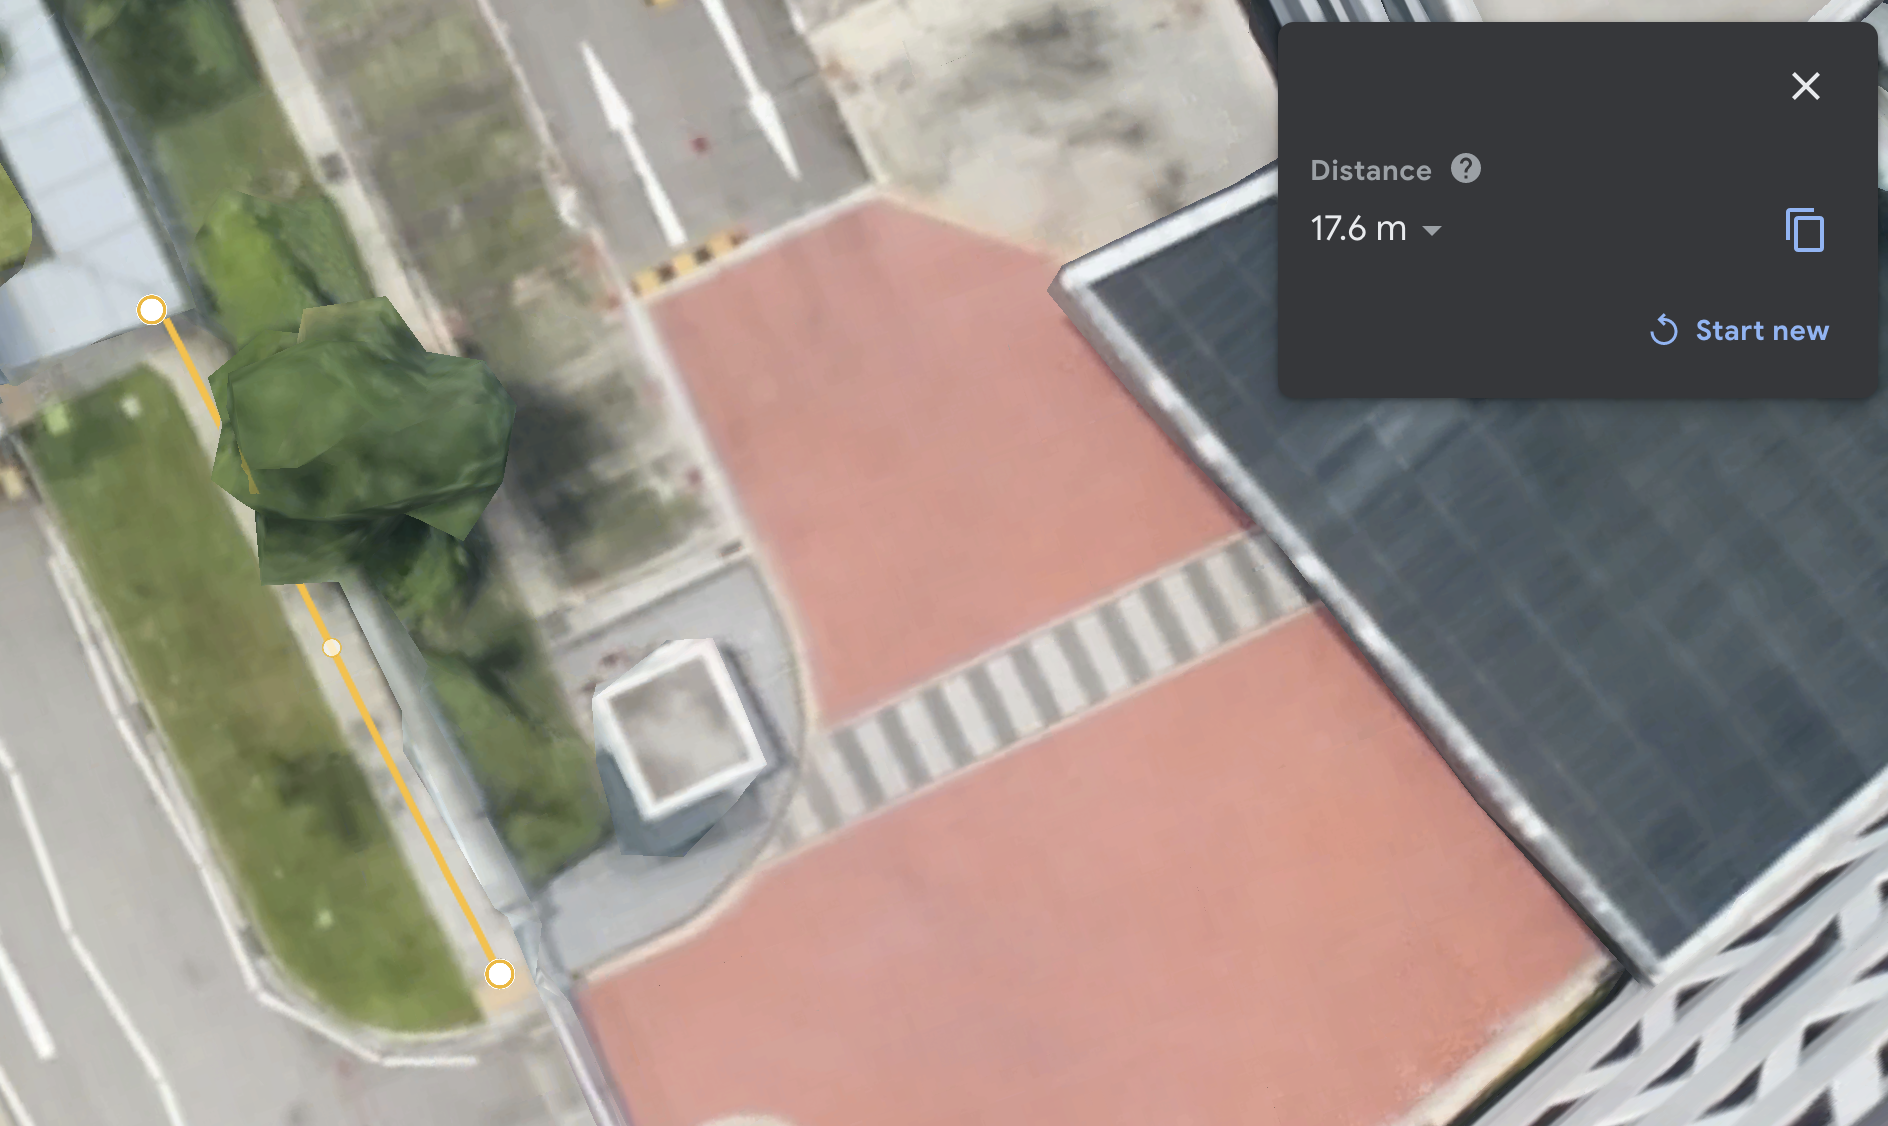
\includegraphics[width=\textwidth]{unshelteredAreaOutsideSst.png}
    \caption{Unsheltered Pathway Outside SST}
    \label{fig:unshelteredAreaOutsideSst}
\end{figure}

\subsubsection{Additional construction-related concerns}

Factors such as constructing lamps for light source along the walkway are not considered as the weight of such trivial details are negligible.

\subsubsection{Graphs for modelling Shelters}

For all graphs displayed in this project to model physical shelters, unless stated otherwise,
\begin{itemize}
    \item The scale is 1 unit to 1 metre.
    \item The ground is flat at $y=0$.
    \item There is no maximum height limit.
    \item All disconnections in piecewise functions like seen in Figure \ref{fig:piecewiseGraph}, are assumed to be vertical flashings. Flashings are vertical connectors between disconnected shelters, like seen in Figure \ref{fig:flashingExample}.
\end{itemize}

\begin{figure}[htbp]
    \centering
    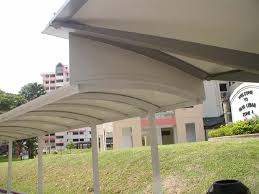
\includegraphics[width=\textwidth]{flashingExample.jpeg}
    \caption{Walkway shelter flashing}
    \label{fig:flashingExample}
\end{figure}

\begin{figure}[htbp]
    \centering
    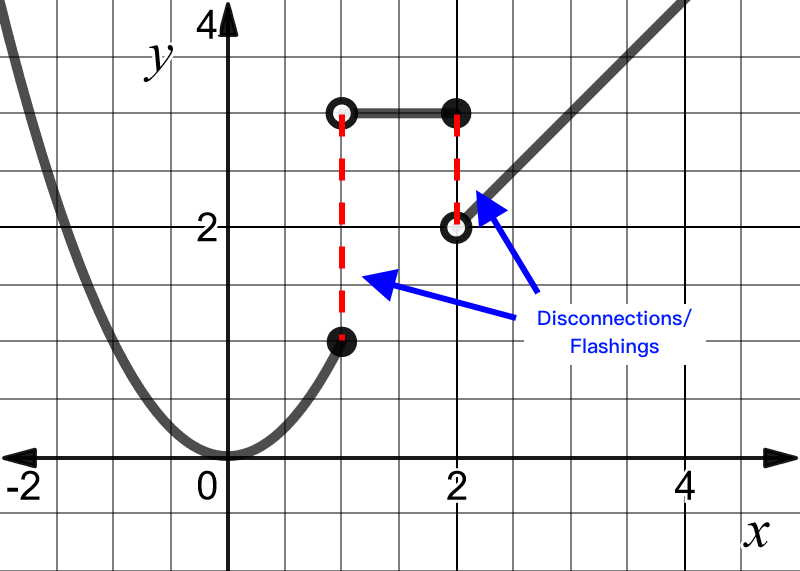
\includegraphics[width=\textwidth]{piecewiseGraph.png}
    \caption{Piecewise graph with annotations}
    \label{fig:piecewiseGraph}
\end{figure}

\subsubsection{Rain velocity}

The rain velocity is directly and solely caused by the wind velocity and not any other factor, thus the rain velocity equals the wind velocity.

\subsection{Simplifications}\label{sec:Assumptions and Simplifications:Simplifications}

\subsubsection{Volume of Shelter}

When calculating the volume of the shelter, the long-side cross-section is taken to be uniform and only that cross-sectional area is utilised in deriving the volume. This simplification is necessary because it is hard to find the volume of a curved 3D plane (requires solving of multi-variable integrals), especially when both functions are modelled by non-linear functions.

\subsubsection{Weight of columns}

\begin{figure}[htbp]
    \centering
    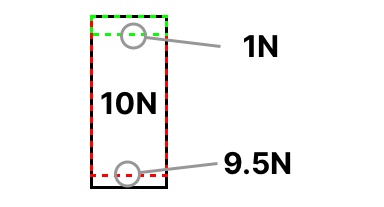
\includegraphics[width=\textwidth]{negligibleWeightOfColumn.png}
    \caption{Illustration of reasoning why weight of columns should be negligible}
    \label{fig:negligibleWeightOfColumn}
\end{figure}

The weight of the material used to construct the columns is considered to be negligible. This simplification is necessary to prevent overcomplication of weight at different parts of the column. For example, the stress applied on the column at higher points is lower than that of the bottom due to the extra weight of the column itself, as seen in Figure \ref{fig:negligibleWeightOfColumn}.

\subsubsection{"Non-Mixture" Materials Used}
The materials used in any example are general examples of the material, meaning specific nuances of the same material are not considered. For instance, there exists many types of steel, like A36 Steel and 1018 Steel. This removes the need of testing too many of the same material like the example stated.

\subsubsection{Short-side cross section positioning}

Since the short-side cross-section of the shelter is modelled independently, the problem can be simplified by ignoring the absolute position at which the polynomial graph is at, only having to take into consideration points on a graph relative to other points on the graph. For instance, a model of a straight line at $y=1$ can be taken as the same shape as a graph at $y=10$, like as seen in Figure \ref{fig:shortSidePosition}.

\begin{figure}[htbp]
    \centering
    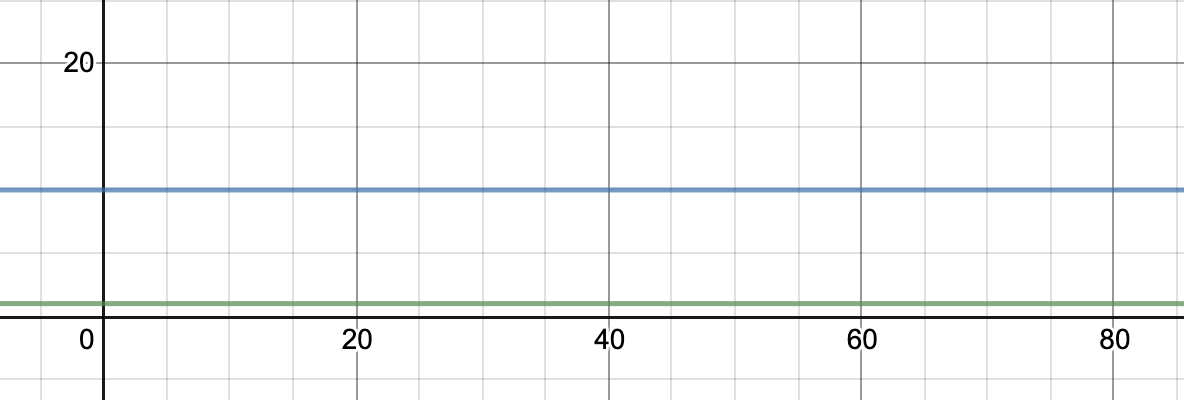
\includegraphics[width=\textwidth]{shortSidePosition.png}
    \caption{Graph of 2 lines which model the same short-side cross-section}
    \label{fig:shortSidePosition}
\end{figure}

\pagebreak
\section{Mathematical Model}\label{sec:Mathematical Model}

\subsection{Rain Water Diversion}\label{sec:Mathematical Model:Rain Water Diversion}

There is generally a standard set of shapes for the short-side cross-sections of walkway shelters, which all have their pros and cons. The various possible models, based these pros and cons, will be weighed in relation to how the shelter may divert rain water that falls on it, and find a optimal function to model the short-side cross-section of the shelter.

The shape of the shelter with design $n$ would be modelled by a polynomial, $f_n(x)$, for $0<x<3$, since the width of the short-side cross-section of the shelter is $3\si{m}$.



There are 2 main issues that need to be considered when selecting the optimal function to model the short-side cross-section of the shelter, which will be explained in further detail later on:

\begin{enumerate}
    \item Water should not get trapped on the shelter.
    \item Water should not slide off the sides too much lest affecting pedestrians' view.
\end{enumerate}

\subsubsection{Flat and Linear}
A flat and linear shelter can be modelled as:
\begin{equation}
    f_1(x)=0
\end{equation}

\begin{tikzpicture}
    \begin{axis}[xlabel=$x$, ylabel=$f_1(x)$, domain=0:3]
        \addplot{0};
    \end{axis}
\end{tikzpicture}

Such a flat and linear shelter with gradient of 0 throughout would mean that
\begin{itemize}
    \item When it is raining, rain would be just as likely to fall off the left than it is to fall off the right.
    \item After it finishes raining, rain might get trapped on top because when the slope is 0, without any force from other droplets of falling as rain, the water droplets would just stay still.
\end{itemize}

As a result of the potential for trapped rain, a flat and linear shelter is not the model for the optimal shelter.

\subsubsection{Quadratic Concave Downwards}
A downwards concave quadratic shelter can be modelled as:

\begin{align}
    f_2(x)&=-0.1(x-0)(x-3)\\&=-0.1x^2+0.3x
\end{align}

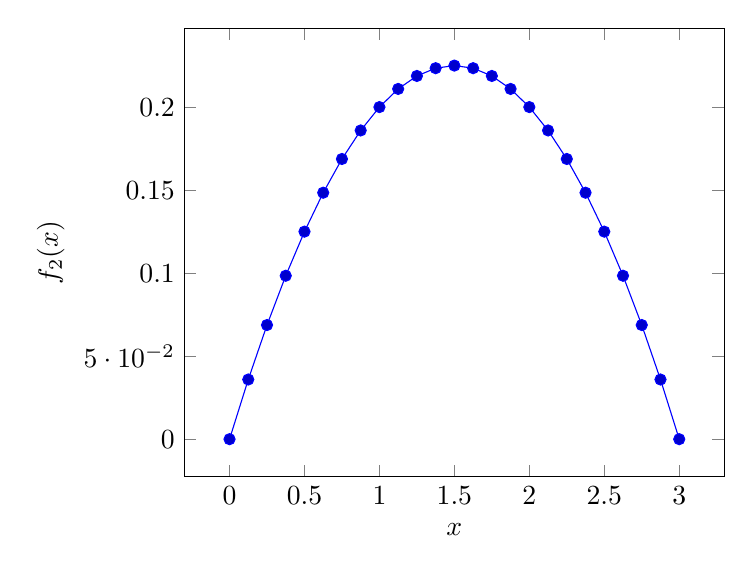
\begin{tikzpicture}
    \begin{axis}[xlabel=$x$, ylabel=$f_2(x)$, domain=0:3]
        \addplot{-0.1*x^2 + 0.3*x};
    \end{axis}
\end{tikzpicture}

When the graph is concave downwards, rain that falls onto the shelter would immediately slide off the 2 sides, with a very low chance of getting stuck on the shelter.

However, the shelter is to be implemented over the crossing of a road. If heavy rain is to fall on both sides of the shelter, it will hinder pedestrians' vision of incoming vehicles, making this design potentially unsafe. However, this design is still logically better than the first one albeit its weaknesses.

\subsubsection{Quadratic Concave Upwards}
A upwards concave quadratic shelter can be modelled as:

\begin{align}
    f_3(x)&=0.1(x-0)(x-3)\\&=0.1x^2-0.3x
\end{align}

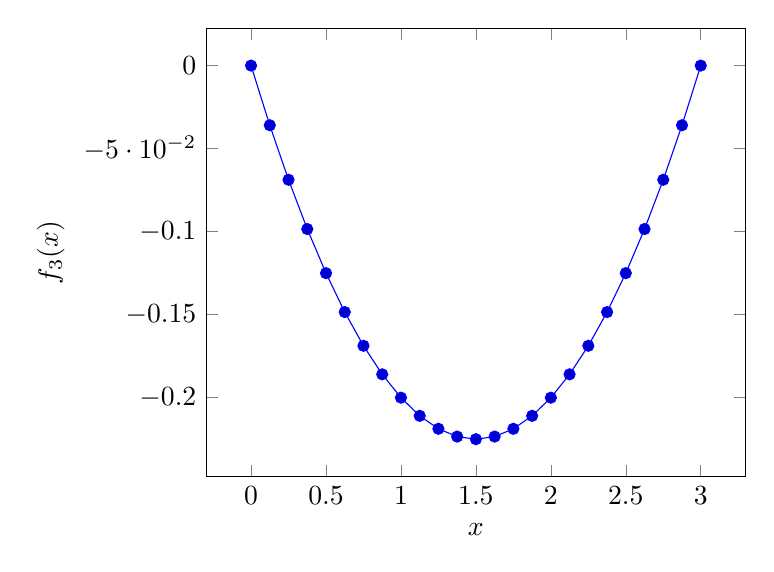
\begin{tikzpicture}
    \begin{axis}[xlabel=$x$, ylabel=$f_3(x)$, domain=0:3]
        \addplot{0.1*x^2 - 0.3*x};
    \end{axis}
\end{tikzpicture}

When the shelter is modelled after a concave upwards graph, water will not fall off to the sides, thus rain will collect in the parabola shaped shelter and eventually flow over. However, with a rain water diversion system for the long-side cross-section of the shelter, this model would work. Ergo, this can be taken into consideration when selecting the optimal function to model the long-side cross-section of the shelter.

\subsection{Rain Angle}\label{sec:Mathematical Model:Rain Angle}

The rain angle is also a crucial factor to the deciding on a optimal design as the principal purpose of a shelter is to block the rain. If the shelter is angled in a way such that rain can still touch pedestrians, then the shelter and its designers have failed.

Hence, the target of this section is to find a better short-side cross-section, while building upon previous models and keeping to the aforementioned aims as well.

Let $\theta$ be the angle of incidence of the rain, or more specifically, the angle between a straight line perpendicular to the ground and the incoming ray, such as rain direction or shelter angle, like seen in Figure \ref{fig:angleOfIncidenceOfRain}. When the angle is measured from the left, it is measured clockwise. When the angle is measured from the right, it is measured anti-clockwise.

\begin{figure}[htbp]
    \centering
    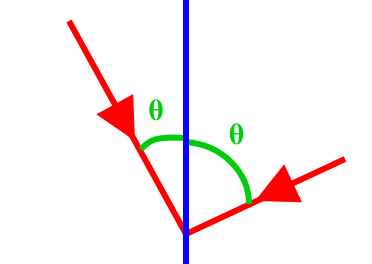
\includegraphics[width=5cm]{angleOfIncidenceOfRain.png}
    \caption{Illustration of angle of incidence of rain}
    \label{fig:angleOfIncidenceOfRain}
\end{figure}

A group of researchers from universities around the world conducted a study on the effect of wind on raindrop impact and rain splash detachment \cite{erpul_darrell_gabriels-rainvelocityangle}. They ``calculated the average rain inclination (a) from vertical and (b) average angle of incidence between the wind vector and the plane of surface as a function of horizontal wind velocity'', as shown in Figure \ref{fig:researchGateRainVelocityAngleGraph}.

\begin{figure}[htbp]
    \centering
    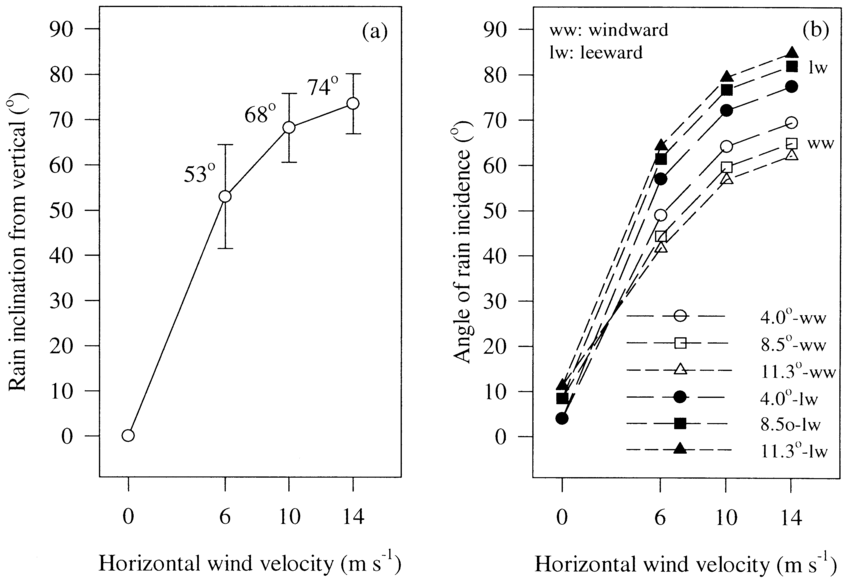
\includegraphics[width=\textwidth]{researchGateRainVelocityAngleGraph.png}
    \caption{Graph of function calculated by researchers investigating the effect of wind on raindrop impact and rain splash detachment}
    \label{fig:researchGateRainVelocityAngleGraph}
\end{figure}

With this function and the estimated mean horizontal wind velocity in Singapore, as stated in the controlled variables, $\theta$ can be estimated using graphical methods as seen in Figure \ref{fig:researchGateRainVelocityAngleGraphAnnotated}, resulting in $\theta_\text{rain}=22\si{\degree}$.

\begin{figure}[htbp]
    \centering
    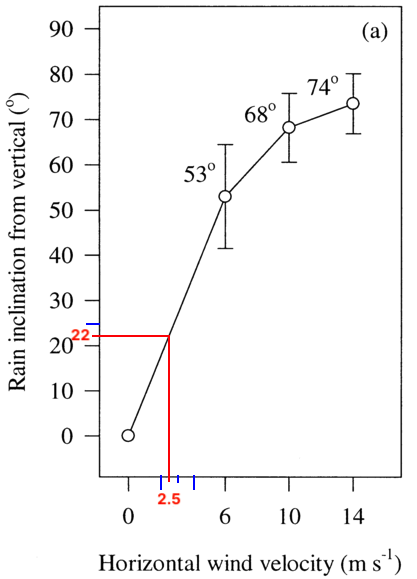
\includegraphics[width=6cm]{researchGateRainVelocityAngleGraphAnnotated.png}
    \caption{Annotated graph of function calculated by researchers investigating the effect of wind on raindrop impact and rain splash detachment}
    \label{fig:researchGateRainVelocityAngleGraphAnnotated}
\end{figure}

\subsubsection{Quadratic Concave Upwards}
As seen in the previous section, the quadratic concave upwards graph was the most optimal design for diverting rain that falls on the shelter.

\begin{align}
    f_3(x)&=0.1(x-0)(x-3)\\&=0.1x^2-0.3x
\end{align}

For either side of the symmetric parabola, $\theta$ can be found as seen in Figure \ref{fig:gradientToAngleGraph}, by first finding the gradient of either ends of the shelter. To do so, the derivative of the function $f_3(x)$, at $x=3$ can be calculated.

\begin{align}
    {f_3}'(x)&=0.2x-0.3\\
    {f_3}'(3)&=0.2(3)-0.3\\
    &=0.3
\end{align}

Since gradient is equals to rise over run, or $\frac{\Delta y}{\Delta x}$, the angle of the gradient in relation to the line perpendicular to the ground, as seen in Figure \ref{fig:gradientToAngleGraph}, can be found.

\begin{figure}[htbp]
    \centering
    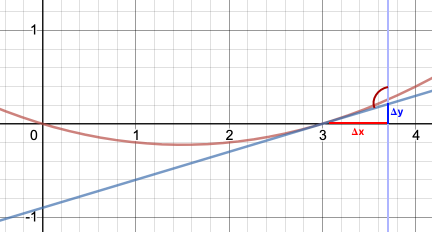
\includegraphics[width=\linewidth]{gradientToAngleGraph.png}
    \caption{Graph of finding the angle of a gradient for $f_3(x)$}
    \label{fig:gradientToAngleGraph}
\end{figure}

\begin{align}
    \cot(180\si{\degree}-\theta)&=\frac{\Delta y}{\Delta x}\\
    180\si{\degree}-\theta&=\arccot\frac{\Delta y}{\Delta x}\\
    \theta&=180-\arccot\frac{\Delta y}{\Delta x}\\
    \theta_3&=180-\arccot0.3\\
    \theta_3&=106.7\si{\degree}&&\text{(4 SF)}
\end{align}

By using logic, it is apparent that a larger angle is worse for pedestrians as more rain pouring in at $22\si{\degree}$ would go under the shelter, making the area for walking smaller. This is illustrated in Figure \ref{fig:rainPourUnderShelter}.

\begin{figure}[htbp]
    \centering
    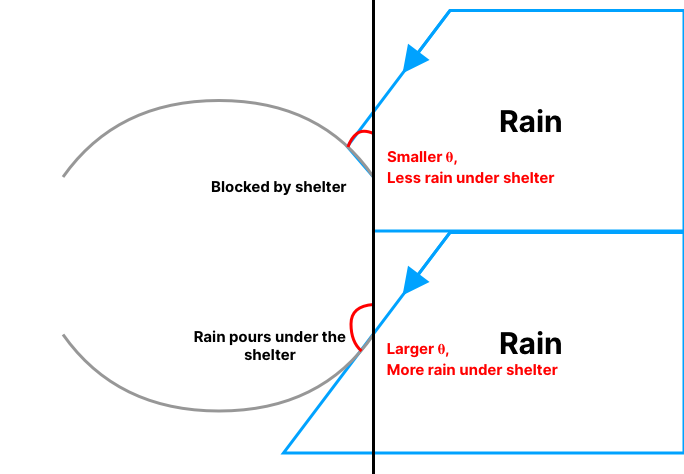
\includegraphics[width=\textwidth]{rainPourUnderShelter.png}
    \caption{More rain pouring under shelter when $theta$ is larger}
    \label{fig:rainPourUnderShelter}
\end{figure}

Consequently, this model can be improved by preventing rain from pouring under the shelter.

\subsubsection{Quartic Concave Upwards}

In order to mitigate the issues detailed above, the short-side cross section of the shelter can be curved at the ends slightly, while still keeping the drain shape to divert the rain water.

\begin{align}
    f_4(x)&=-0.1(x-0)(x-1.5)(x-1.5)(x-3)\\
    &=-0.1x^4+0.6x^3-1.125x^2+0.675x
\end{align}

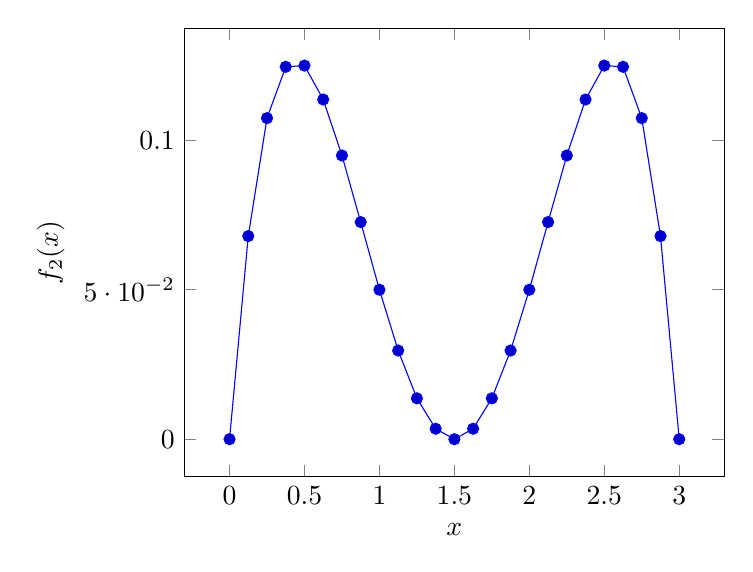
\begin{tikzpicture}
    \begin{axis}[xlabel=$x$, ylabel=$f_2(x)$, domain=0:3]
        \addplot{-0.1*x^4 + 0.6*x^3 - 1.125*x^2 + 0.675*x};
    \end{axis}
\end{tikzpicture}

As with the previous model, $\theta$ of the shelter at its ends can be found by taking the derivative at $x=3$.

\begin{align}
    {f_4}'(x)&=0.675-2.25x+1.8x^2-0.4x^3\\
    {f_4}'(3)&=0.675-2.25(3)+1.8(3)^2-0.4(3)^3\\
    &=-0.675
\end{align}

Using the formula previously derived for $\theta$,

\begin{align}
    \theta&=180-\arccot\frac{\Delta y}{\Delta x}\\
    \theta_4&=180-\arccot(-0.675)\\
    \theta_4&=56.00\si{\degree}&&\text{(4 SF)}
\end{align}

As seen above, $\theta$ is much smaller, thus this model has solved the issue of the rain angle.

\subsection{Vehicle Passing-Through}\label{sec:Mathematical Model:Vehicle Passing-Through}

Traditionally, there is also a conventional set of structures for the long-side cross-sections of walkway shelters, which all have their pros and cons. The various possible models, based these pros and cons, will be weighed in relation to how the shelter may allow for a vehicle of reasonable size to pass through, and find a optimal function to model the long-side cross-section of the shelter.

The shape of the shelter with design $n$ would be modelled by a polynomial, $g_n(x)$, for $0<x<21.5$, since the length of the long-side cross-section of the shelter is $21.5\si{m}$.

Any model should fulfill these required controlled variables:
\begin{enumerate}
    \item Passes through y-intercept of 1.5 (Height of school gate)
    \item Passes through $y=4$, when $x\ge21.5$ (Height of shelter)
    \item For $8.8<x<21.5$, $y\ge5.0$
\end{enumerate}

There are 3 key issues to address when selecting the optimal function to model the long-side cross-section of the shelter, which will be explained in further detail later on:

\begin{enumerate}
    \item Allows for diverting flow of rain water (from previous section).
    \item Allows vehicles of cross-sectional areas of height $5.0\si{m}$ and width $3.1\si{m}$ to pass under.
    \item Water should not get trapped on the shelter.
\end{enumerate}

\subsubsection{Linear discontinuous}
A linear modelled shelter with vertical flashings or columns, would be similar to the shelter right outside of SST like seen in Figure \ref{fig:shelterOutsideSst}.

\begin{figure}[htbp]
    \centering
    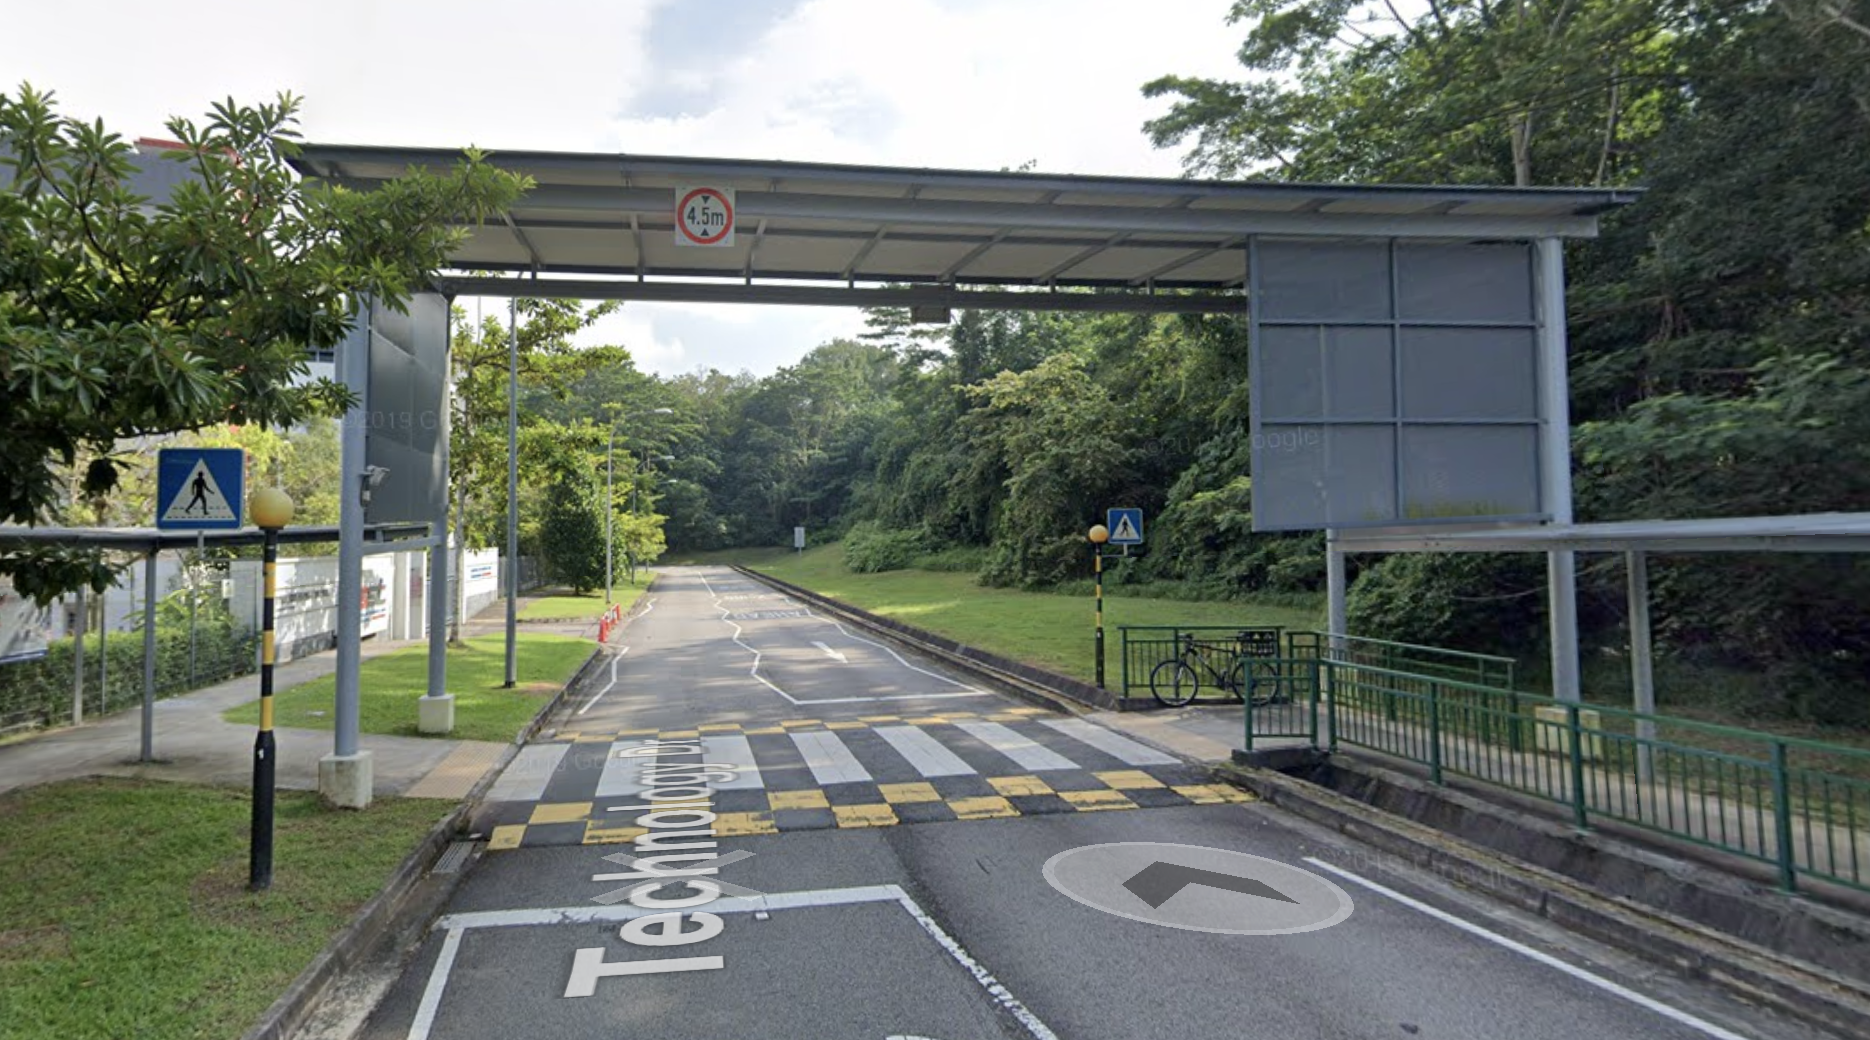
\includegraphics[width=\textwidth]{shelterOutsideSst.png}
    \caption{Shelter outside SST}
    \label{fig:shelterOutsideSst}
\end{figure}

This shelter design can be modelled by a piecewise linear function as seen in Figure \ref{fig:linearDiscontinuousGraph}, where all the discontinuities are assumed to be vertical flashings (vertical connectors between shelters), or columns to support the shelter:

\begin{align}
    g_1(x)&=\begin{cases} 
      x<8.8 & x\leq 2.5 \\
      x<21.5 & 5
   \end{cases}
\end{align}

\begin{figure}[htbp]
    \centering
    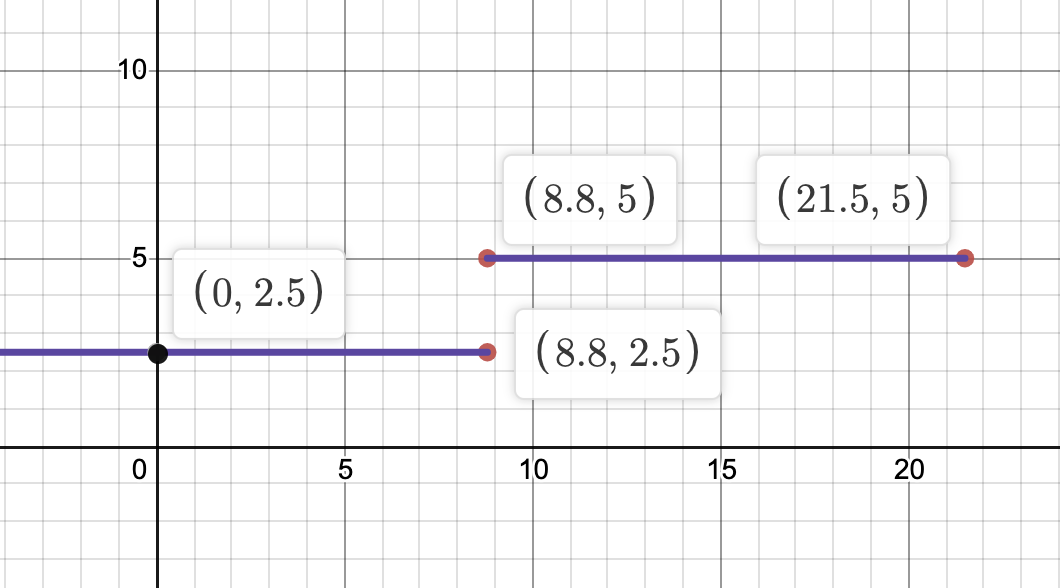
\includegraphics[width=\textwidth]{linearDiscontinuousGraph.png}
    \caption{Graph of linear discontinuous model}
    \label{fig:linearDiscontinuousGraph}
\end{figure}

However, this design is not optimal because it fulfills only 1 of the previously stated goals, not allowing for diverting flow of rain water and water might still get trapped on the shelter. Because of the flat design, water would have no specific direction to flow towards.

\subsubsection{Downwards Concave}

In order to find a downwards concave quadratic equation that fulfills the requirements stated above, more calculations are required. The rough idea of how the shelter would look like in context can be seen in Figure \ref{fig:downwardsConcaveRoughIdea}.

\begin{figure}[htbp]
    \centering
    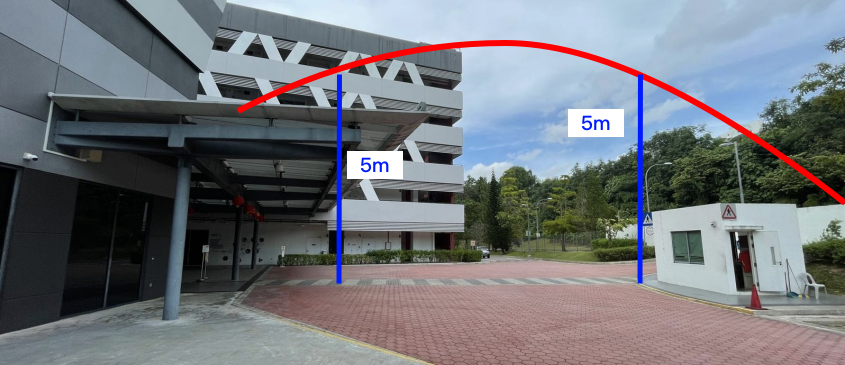
\includegraphics[width=\textwidth]{downwardsConcaveRoughIdea.png}
    \caption{Rough idea of how a downwards quadratic model would fit}
    \label{fig:downwardsConcaveRoughIdea}
\end{figure}

To begin finding the equation to model this design, the graph with points plotted is sketched, as seen in Figure \ref{fig:downwardsConcaveSketch}.

\begin{figure}[htbp]
    \centering
    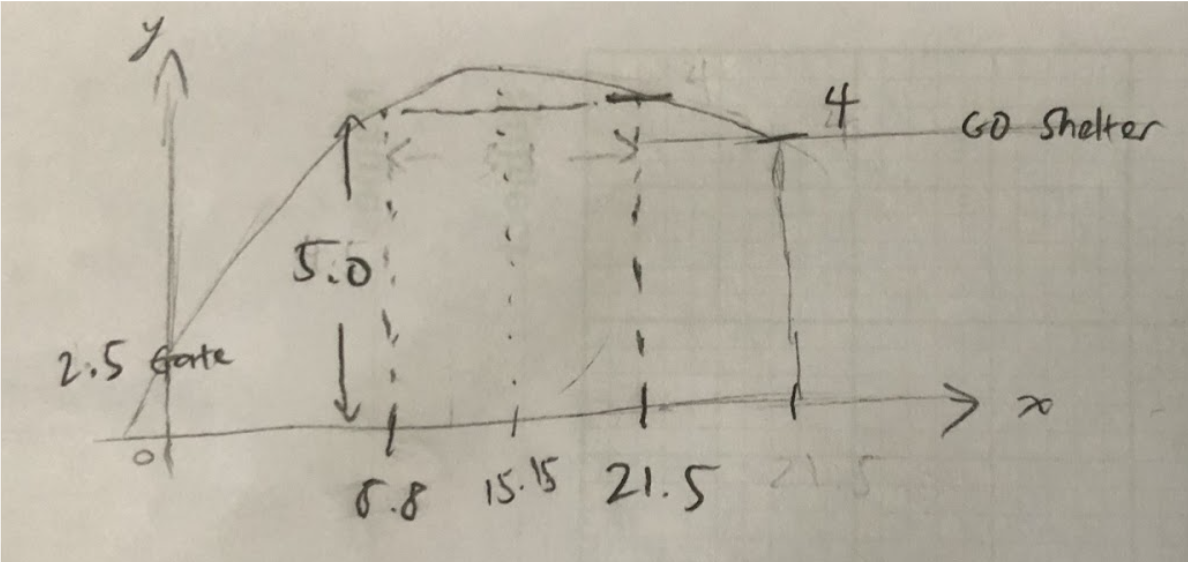
\includegraphics[width=\textwidth]{downwardsConcaveSketch.png}
    \caption{Rough idea of how a downwards quadratic model would fit}
    \label{fig:downwardsConcaveSketch}
\end{figure}

After sketching the graph, it is obvious that by using the 2 points of intersection of the graph with the line $y = 5$, line of symmetry can be found. Then, the equation can be plugged into the vertex form ($y=a(x-p)(x-q)$) and converted into the standard form ($y=ax^2+bx+c$). By comparison, $k$ can be substituted out, leaving one variable, $a$, which can be solved for. After obtaining $a$, substituting back into the original equation allows us to find the equation of the graph:

\begin{align}
    g_2(x)&=\left(-\frac{25}{1892}\right)x^{2}-\frac{303}{10}\left(-\frac{25}{1892}\right)x+2.5
\end{align}

\begin{figure}[htbp]
    \centering
    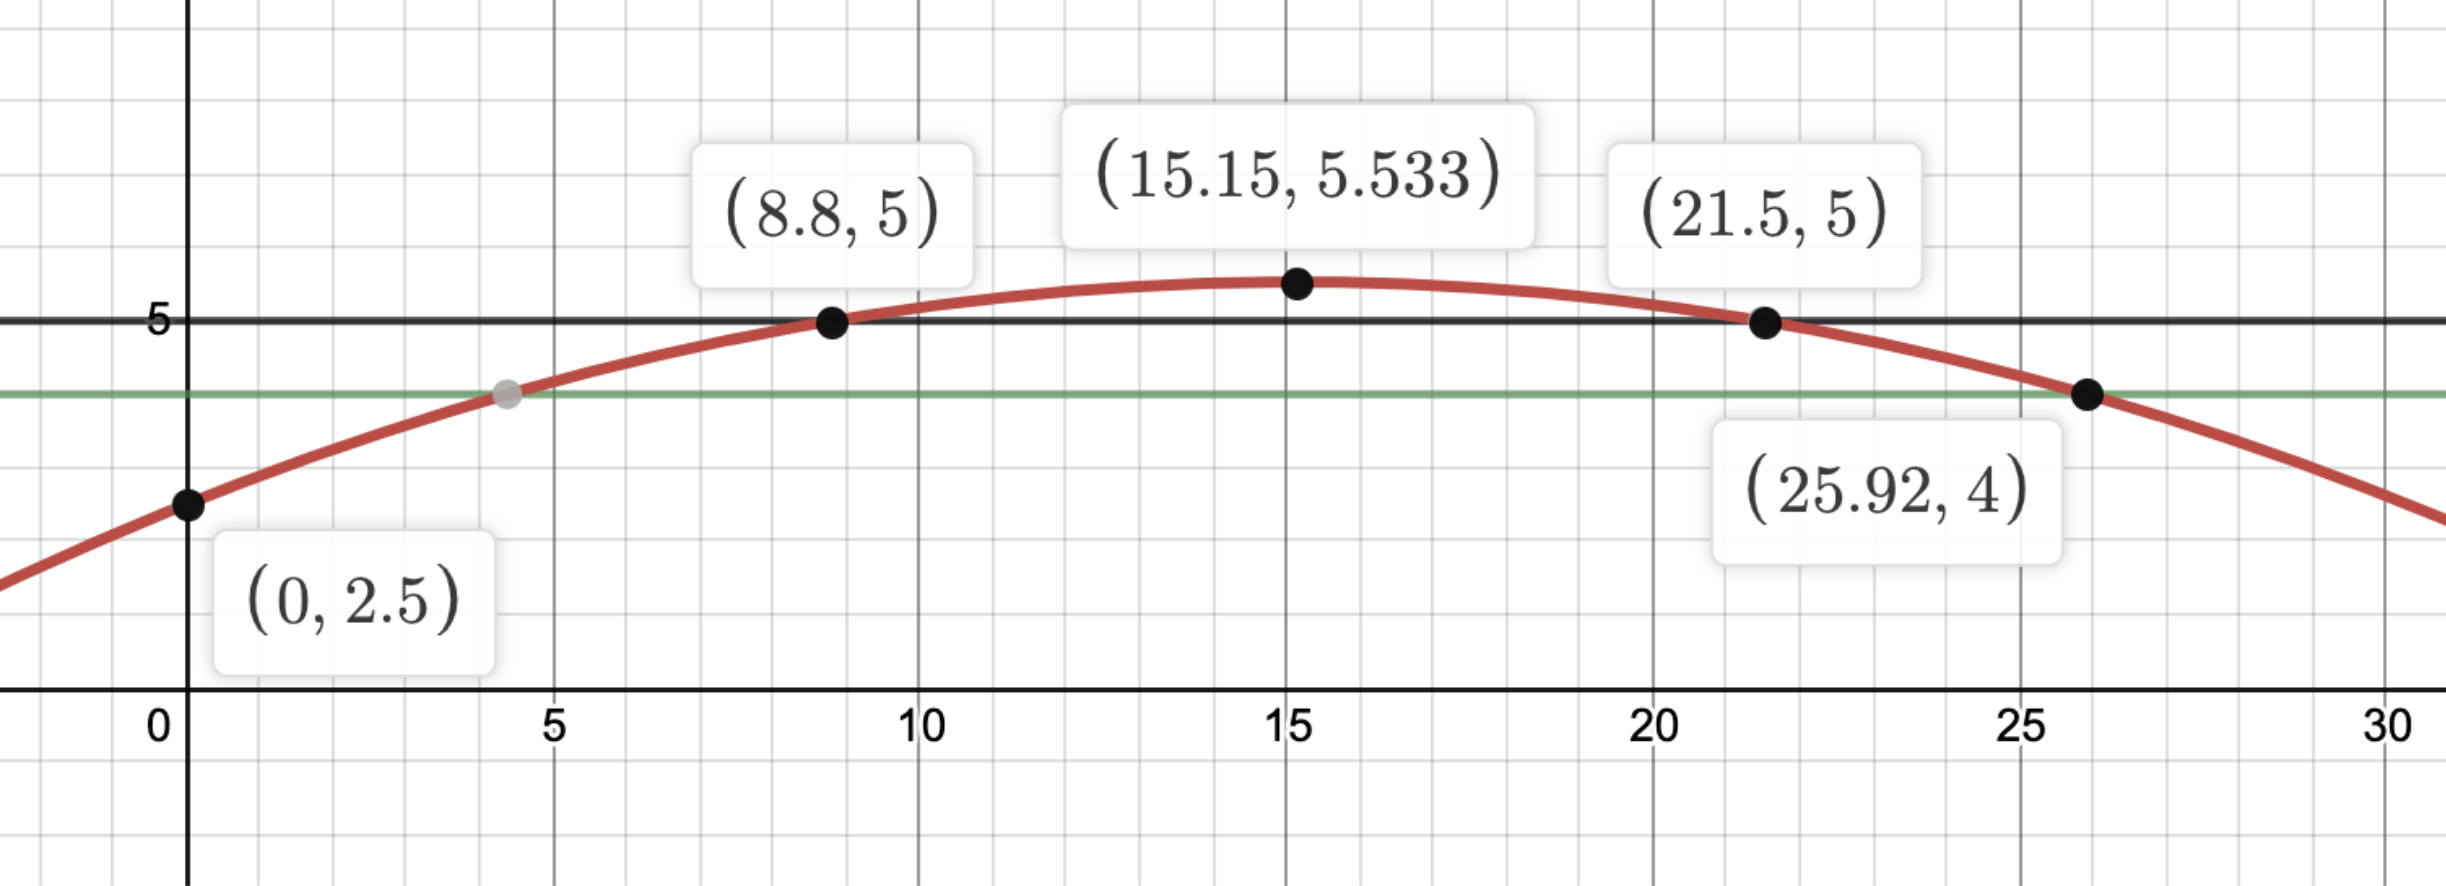
\includegraphics[width=\textwidth]{downwardsConcaveGraph.png}
    \caption{Graph of downwards concave quadratic model}
    \label{fig:downwardsConcaveGraph}
\end{figure}

The full derivation of the equation above can be found below:

\begin{gather}
    y=a(x-h)^2+k\\
    y=a(x-\frac{303}{20})^2+k\\
    y=a(x^2-\frac{303}{10}x+(\frac{303}{20})^2)+k\\
    y=y=ax^2-\frac{303}{10}ax+(\frac{303}{20})^2+k\\
    \because y=ax^2+bx+c\\
    c=(\frac{303}{10})^2+k\\
    y=ax^2-\frac{303}{10}ax+2.5\\
    \text{When }@(8.8, 5.0)\\
    5=8.8^2a-\frac{303}{10}(8.8)a+2.5\\
    -\frac{946}{5}a=2.5\\
    a=-\frac{25}{1892}\\
    \therefore y=\left(-\frac{25}{1892}\right)x^{2}-\frac{303}{10}\left(-\frac{25}{1892}\right)x+2.5
\end{gather}

This quadratic downwards concave graph is a somewhat optimal solution to the long-side cross section of the shelter. This is because it fulfills all 3 of the previously stated goals which were:

\begin{enumerate}
    \item Allows for diverting flow of rain water (from previous section).
    \item Allows vehicles of cross-sectional areas of height $5.0\si{m}$ and width $3.1\si{m}$ to pass under.
    \item Water should not get trapped on the shelter.
\end{enumerate}

With this model, water would slide down either side of the polynomial, where water can be collected in a pipe and directed into a drain on the ground, thus also solving the problem in the previous section.

\subsection{Materials Used}\label{sec:Mathematical Model:Materials Used}

\subsubsection{Material of Shelter Cover}

By deciding on a suitable material for the shelter's cover, the required strength of the supporting columns can be determined.

Using the arc length formula \cite{mathisfun-arclength}:

\begin{equation}
    S=\int_a^b\sqrt{1+(f'(x))^2}dx
\end{equation}

The volume of the shelter can be estimated by finding $\text{Shelter Volume}=\text{Arc Length}\cdot\text{Shelter short-side Cross Sectional Area}$.

\begin{align}
    g_2(x)&=\left(-\frac{25}{1892}\right)x^{2}-\frac{303}{10}\left(-\frac{25}{1892}\right)x+2.5\\
    g_2'(x)&=-\frac{25}{946}x+\frac{1515}{3784}\\
    \text{Arc Length}&=\int_0^{25.92}\sqrt{1+(g_2'(x))^2}dx\\
    &=29.46&&\text{(4 SF)}\\
    \text{Volume of Shelter}&=29.46\cdot3.0\cdot0.01\\
    &=0.8838\si{m^3}
\end{align}

Given the volume of the shelter to be $0.8838\si{m^3}$, the weight of the shelter built with a given material, $M$, can be found. Density, $\rho$, is defined as mass, $m$, per unit volume, $V$ ($\rho=\frac{m}V$), and weight, $W$, is defined as the product of mass, $m$, and gravitational acceleration, $g$ ($W=mg$). The densities of the materials found via online research papers or websites that have done prior research \cite{anupoju-density}. With this data, the weight of the shelter built with $M$ using the following formula can be found:

\begin{align}
    \rho&=\frac{m}V\\
    m&=\rho V\\
    W&=mg\\
    W_M&=\rho Vg
\end{align}

\begin{table}[htbp]
    \centering
    \begin{tabular}{l|c|c}
        $M$ & $\rho$ ($\si{kg/m^3}$) & $W$ ($\si{N}$) \\
        \hline
        Glass & 2580 & 22369 \\
        Steel & 7850 & 68060 \\
        Aluminium & 2739 & 23747 \\
        Polyvinyl Chloride (Plastic, PVC) & 1380 & 11965 \\
    \end{tabular}
    \caption{Table of plausible materials for the shelter cover}
    \label{tab:shelterCoverMaterial}
\end{table}

Obviously, the most optimal solution would be the lightest material. Therefore, the most optimal solution would be the plastic (PVC), weighing a total of $11965\si{N}$

\subsubsection{Material of Supporting Column}

Ultimate tensile strength, $\sigma$ is defined as the maximum force acting upon a material, $F$, per cross-sectional area, $A$, before failure ($\sigma=\frac{F}A$).

It is a measure of the maximum amount of stress a material can bear before failure \cite{velling-uts}. This is a significant indicator in the success of the shelter. If the shelter is too heavy and cannot be supported by the columns, it would collapse and be a disaster. Therefore, selecting a material with a high ultimate tensile strength is important from the plausible list of materials below.

As stated above in the controlled variables, the cross-sectional area of the column is assumed to be $0.13\si{m^2}$.

The ultimate tensile strength, $\sigma$, for a given material, $M$, can be found via online research papers or websites that have done prior experiments. With this data, the max withstandable force, $F$, of the column made of material, $M$, for a cross-sectional area of $0.13\si{m^2}$, can be calculated with the formula below.

\begin{align}
    \sigma&=\frac{F}A\\
    F&=\sigma A\\
    F_M&=0.13\sigma
\end{align}

\begin{table}[htbp]
    \centering
    \begin{tabular}{l|c|c}
        $M$ & $\sigma$ ($\si{MPa}$) & $F$ ($\si{N}$) \\
        \hline
        Glass & 7 & $8.4\cdot10^5$ \\
        Steel & 420 & $5.04\cdot10^7$ \\
        Aluminium & 90 & $1.08\cdot10^7$ \\
        Polyvinyl Chloride (Plastic, PVC) & 62 & $7.44\cdot10^6$ \\
    \end{tabular}
    \caption{Table of plausible materials for the column}
    \label{tab:columnMaterial}
\end{table}

Clearly, the most optimal solution would be the strongest material. Therefore, the most optimal solution would be Steel, having an ultimate tensile strength of $5.04\cdot10^7\si{N}$.

\subsubsection{Tessellation Material Efficiency}

To create a design that matches the aesthetics of the shelter from which the project took inspiration from, as seen in Figure \ref{fig:downwardsConcaveInspiration}, a tessellated frame to hold the cover is required. Apart from aesthetics, this also acts as additional support to the weight of the cover and force of the rain.

Therefore, different shapes, $S$, and their material efficiency in order to reduce volume of materials required, which ultimately reduces to construction costs, will be compared.

Material efficiency is defined as the amount of material required to create a tessellation of a given shape, and hence, the top surface area of the frame, $A_\text{total}$, which determines the construction costs.

To calculate $A_\text{total}$, the total top-view surface area of the shelter cover is subtracted from the total area of the sum of tessellation shapes, $A_\text{cover}-A_\text{shapes}$.

Three shapes, namely circles, triangles and hexagons, are considered as frame tessellations, to determine material efficiency.

The same concept was then applied to the rest of the shapes. The formula used for calculating the pressure is as follows:

\begin{align}
    A_\text{total}&=A_\text{cover}-A_\text{shapes}
\end{align}

\begin{table}[htbp]
    \centering
    \begin{tabular}{l|c p{5cm}}
        $S$ & $A_\text{total}/\si{cm^2}$ \\
        \hline
        Circle & 70675\\
        Triangle & 66960\\
        Hexagon & 43385\\
    \end{tabular}
    \caption{Table of feasible shapes for lattice structure of shelter}
    \label{tab:latticeStructure}
\end{table}

From the results, it is clear that the hexagon is the most material efficient, as it had the least amount of top surface area.

Hexagons have also mathematically be proven to have the most efficient perimeter-to-area ratio by Thomas C. Hales in his 1999 paper "Honeycomb Conjecture" \cite{hales-honeycomb}. A full explanation has been provided in Elliot's report linked below.

\pagebreak
\section{Other Feasible Models}\label{sec:Other Feasible Models}

This section aims to compare and contrast the different designs by team members, to decide on the best possible design based on the team’s data analysis, research and assumptions.

Based on the conclusions from weighing various designs, the pros of other designs are brought back to the main project for improvements.

\subsection{Elliot's Design}\label{sec:Other Feasible Models:Elliot's Design}

The full report for Elliot's design can be found at \url{https://docs.google.com/presentation/d/1zyhsfGaWW51uiVQ1r5pUjlIV8CNBk3dhaddlZz5BfXE/}.

\subsubsection{Assumptions and Simplifications}

The assumptions made in Elliot's design include:

\begin{itemize}
    \item Factors such as putting lights along the walkway were not considered. Hence, accounting for wiring was not needed and no wire casings will be needed to be in the models.
    \item Emergency vehicles such as fire engines did not need to travel underneath. This is because there other access points to the school’s various blocks other than the teacher’s car parks
    \item Ground is flat throughout and not sloped. This makes for easier calculations when determining dimensions of the walkway
    \item All car heights will not be above 2.5m. This was assumed based on the average carpark height in Singapore
    \item When drawing the graph, it was assumed that the ground is flat and is the x-axis. It was also assumed that the scale is 5 : 1m
\end{itemize}

The simplifications made in Elliot's design include:

\begin{itemize}
    \item Assumed 3m is sufficient for the width of a walkway. This simplifies the problem and makes calculations easier
    \item Rain will fall perpendicularly to the ground. Hence, the walkway will be unable to block rain if the rain falls beyond a certain angle. Certain parts underneath the walkway will then be susceptible to rain
\end{itemize}

\subsubsection{Shape of Shelter}

Elliot's final design is a flat cover tilted at an angle. A flat-roofed design was inspired by LTA's walkways with a similar design with across the island. Such a design would integrate well with SST's generally geometric construction compared to a curved shelter. 

\begin{figure}[htbp]
    \centering
    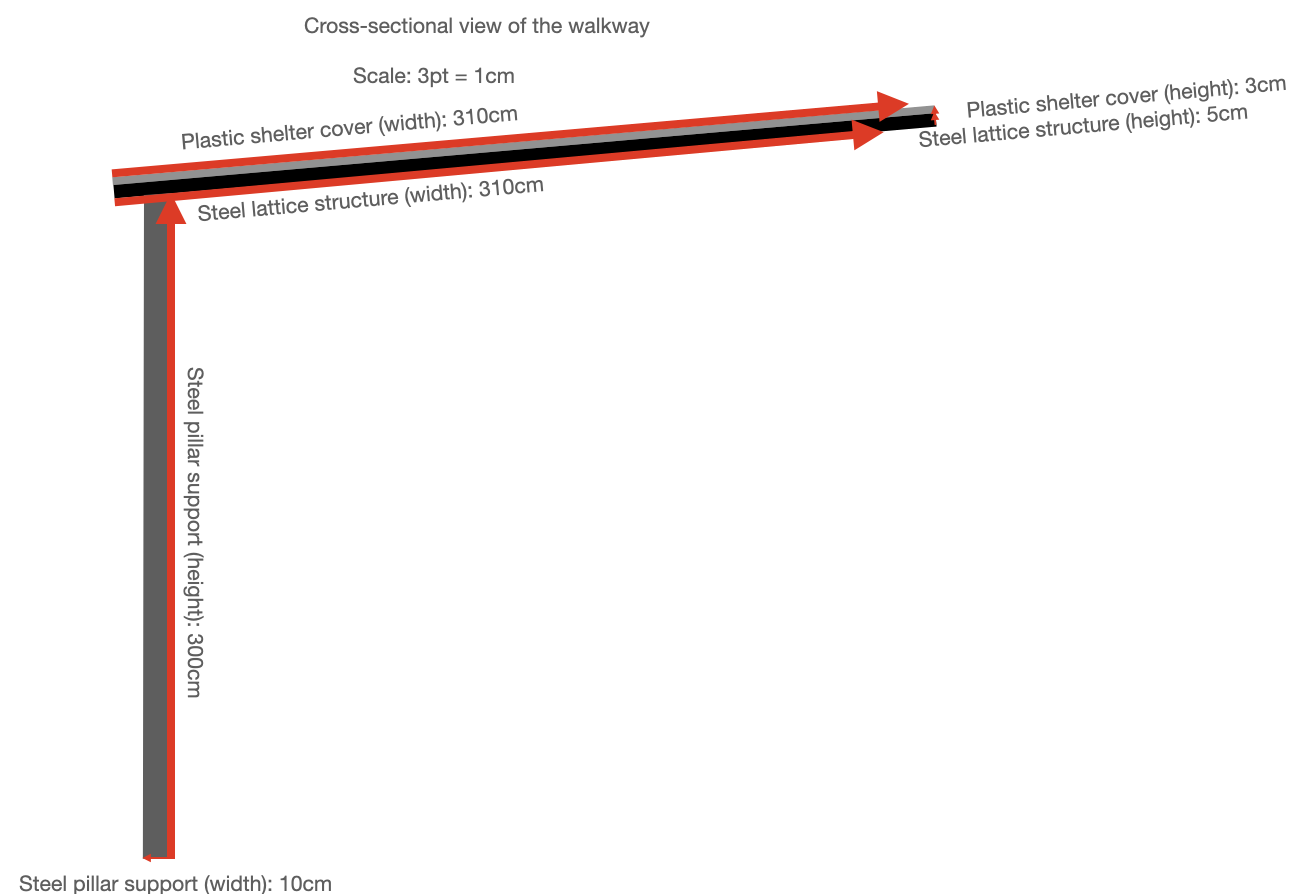
\includegraphics[width=\textwidth]{elliotDesign1.png}
    \caption{Shape of Elliot's final design}
    \label{fig:elliotDesign1}
\end{figure}

\subsubsection{Shape of Lattice for shelter}

Elliot's final design cover is supported by a hexagonal latticed structure. It serves as a frame to support the cover. This hexagonal structure is inline with SST’s theme and usage of hexagons as an icon. Hexagons also have the most efficient perimeter-to-area ratio of any regular polygon that is able to tessellate, hence making it the most material efficient shape to use. 

\begin{figure}[htbp]
    \centering
    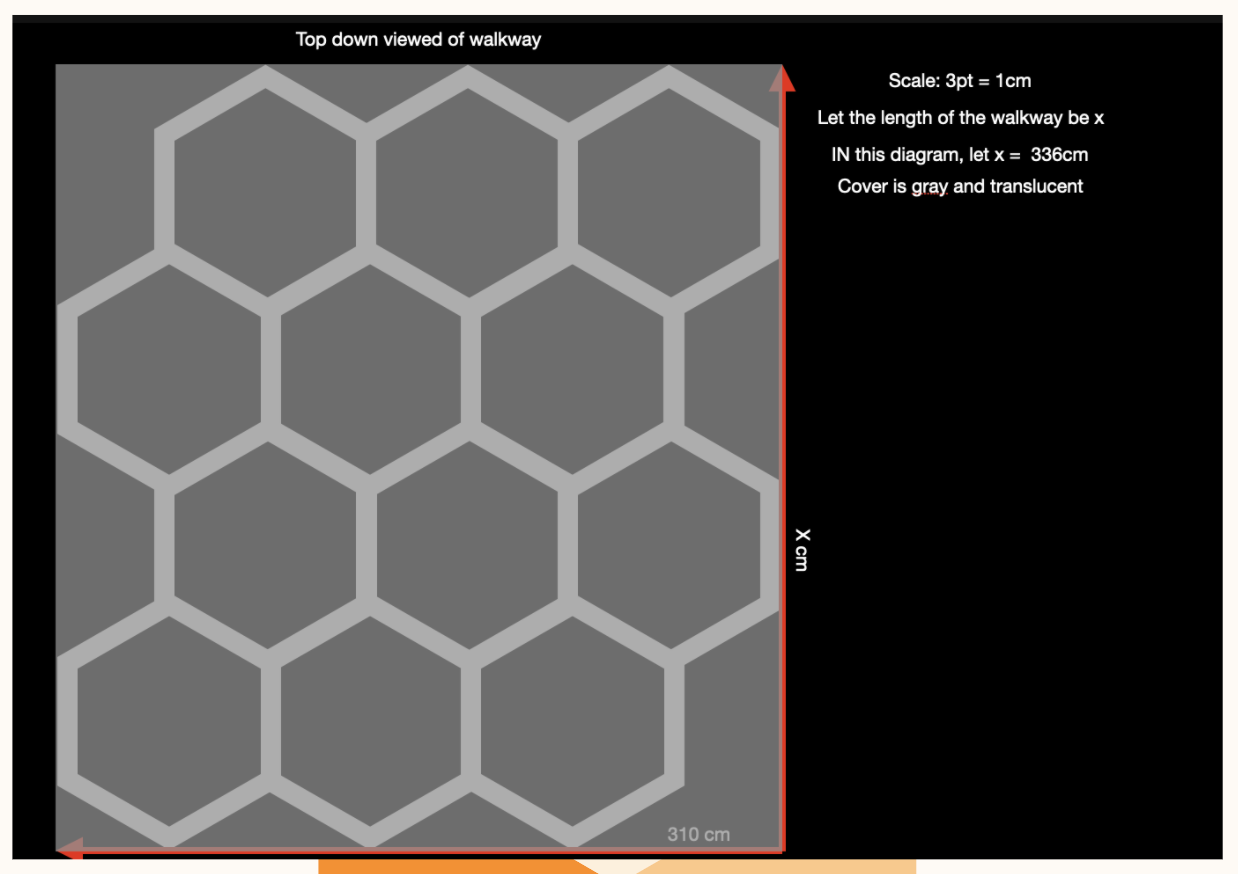
\includegraphics[width=\textwidth]{elliotDesign2.png}
    \caption{Lattice structure of Elliot's final design}
    \label{fig:elliotDesign2}
\end{figure}

\pagebreak

\subsection{Xavier's Design}\label{sec:Other Feasible Models:Xavier's Design}

The full report for Xavier's design can be found at \url{https://docs.google.com/document/d/1qsbObHMt91Q8ieCGMJQ0VPXqUyxONH9n7WiD8RtcQiA/}.

\subsubsection{Assumptions and Simplifications}

The assumptions made in Xavier's design include:

\begin{itemize}
    \item The weight of the concrete used in the support columns is negligible.
    \item The walkway only needs to reach the gates of the school.
    \item The weight of lighting on the walkway is negligible.
\end{itemize}

The simplifications made in Xavier's design include:

\begin{itemize}
    \item The curvature of the roof does not add to weight.
    \item The hexagonal structure is able to support the weight of the roof.
\end{itemize}

\subsubsection{Shape of Shelter}

Xavier's final design includes a curved structure for the roof and has a transparent roof with hexagonal support structures. The structure is supported by circular support columns. The equation for the quadratic graph of the roof is \begin{equation}f(x)=-0.2(x-1.5)^2+5.\end{equation} 

\begin{figure}[htbp]
    \centering
    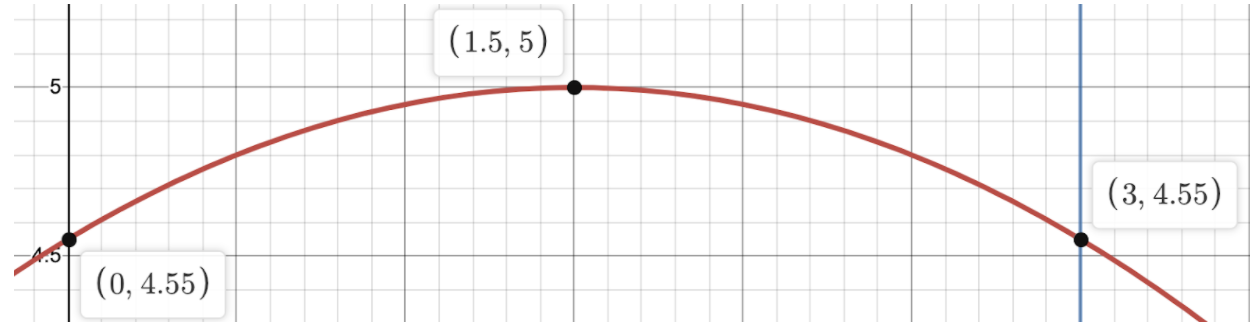
\includegraphics[width=\textwidth]{xavierDesign2.png}
    \caption{Graph of Xavier's final design}
    \label{fig:xavierDesign2}
\end{figure}

The model utilises a quadratic curve for the roof, which allows rainwater to flow off the sides without collecting on top. According to NEA \cite{nea-dengue}, the number of dengue cases is on the rise. Hence, reducing the amount of stagnant water for mosquitoes to breed is important, especially in a school environment, as seen in Figure \ref{fig:dengueCases}.

\subsubsection{Shape of shelter lattice}

Similar to Elliot's design, Xavier's design also comprises of hexagon tiles as the lattice. This lattice of hexagons serves to provide support for the transparent covering of the roof. Hexagons were chosen as it matches SST's theme, as well as being relatively material efficient to ensure maximum material efficiency.

\begin{figure}[htbp]
    \centering
    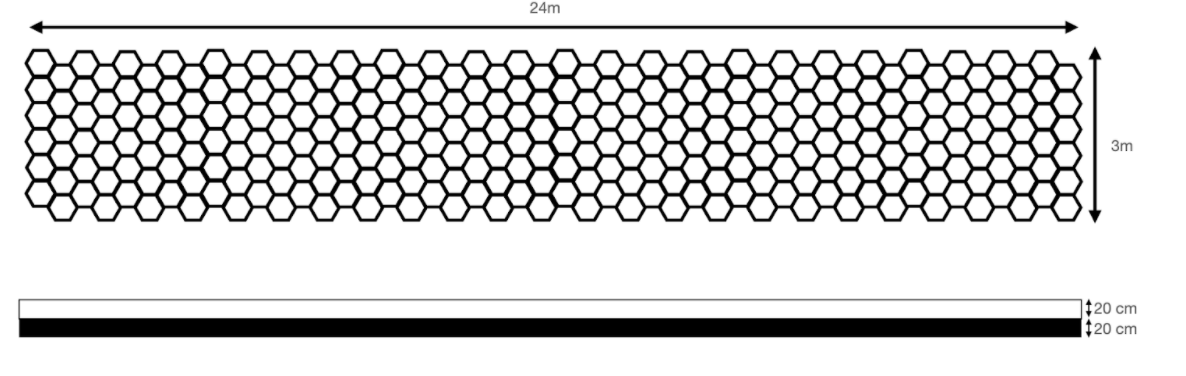
\includegraphics[width=\textwidth]{xavierDesign1.png}
    \caption{Lattice structure of Xavier's final design}
    \label{fig:xavierDesign1}
\end{figure}
\subsubsection{Roof material}

Utilising a transparent material as the main roof material will allow natural sunlight to be used as a lighting source rather than using electrical lights, which will help reduce energy consumption.

\subsubsection{Curve of roof}

The quadratic curve of the roof allows rainwater to flow off easily and prevents stagnant water from collecting. As previously stated, this is important as the number of dengue cases has increased more than two times between 2019 and 2020 \cite{nea-dengue}, as seen in Figure \ref{fig:dengueCases}. Dengue mosquitoes rely on stagnant water to breed. Hence, it is important to allow water to have a place to flow to.

\subsection{Zhi Bing's Design}\label{sec:Other Feasible Models:Zhi Bing's Design}

The full report for Zhi Bing's design can be found at \url{https://docs.google.com/document/d/1SlRSctS6nJvy7HA9-B45OKuUZy401Ant2yzmKFNI6jE/}.

\subsubsection{Assumptions and Simplifications}

The assumptions made in Zhi Bing's design include:

\begin{itemize}
    \item The structure will be able to be supported by the ground.
    \item The shelter is sufficient enough to block any rain that is falling.
    \item The cost of the shelter will be within budget to be covered by the school.
\end{itemize}

The simplifications made in Zhi Bing's design include: 

\begin{itemize}
    \item The shelter can be a parabolic curve.
    \item The shelter need not reach out of the school, sheltering students until the school gate is sufficient.
\end{itemize}

\subsubsection{Shape of Shelter}

Viewed from the front, Zhi Bing's design has a curved roof supported at each end of the footpath by pillars, as seen in Figure \ref{fig:zhiBingDesign}. It enables rain to slide off the end easily thus stagnant water would be absent. It is also considerably wider than the footpath to allow for easier travel for a large number of students, the width of the footpath is 3.0m as seen in Figure \ref{fig:shelterWidth}, the width of the shelter is 5m. The shelter is tall to allow for vehicles to pass below.

\begin{figure}[htbp]
    \centering
    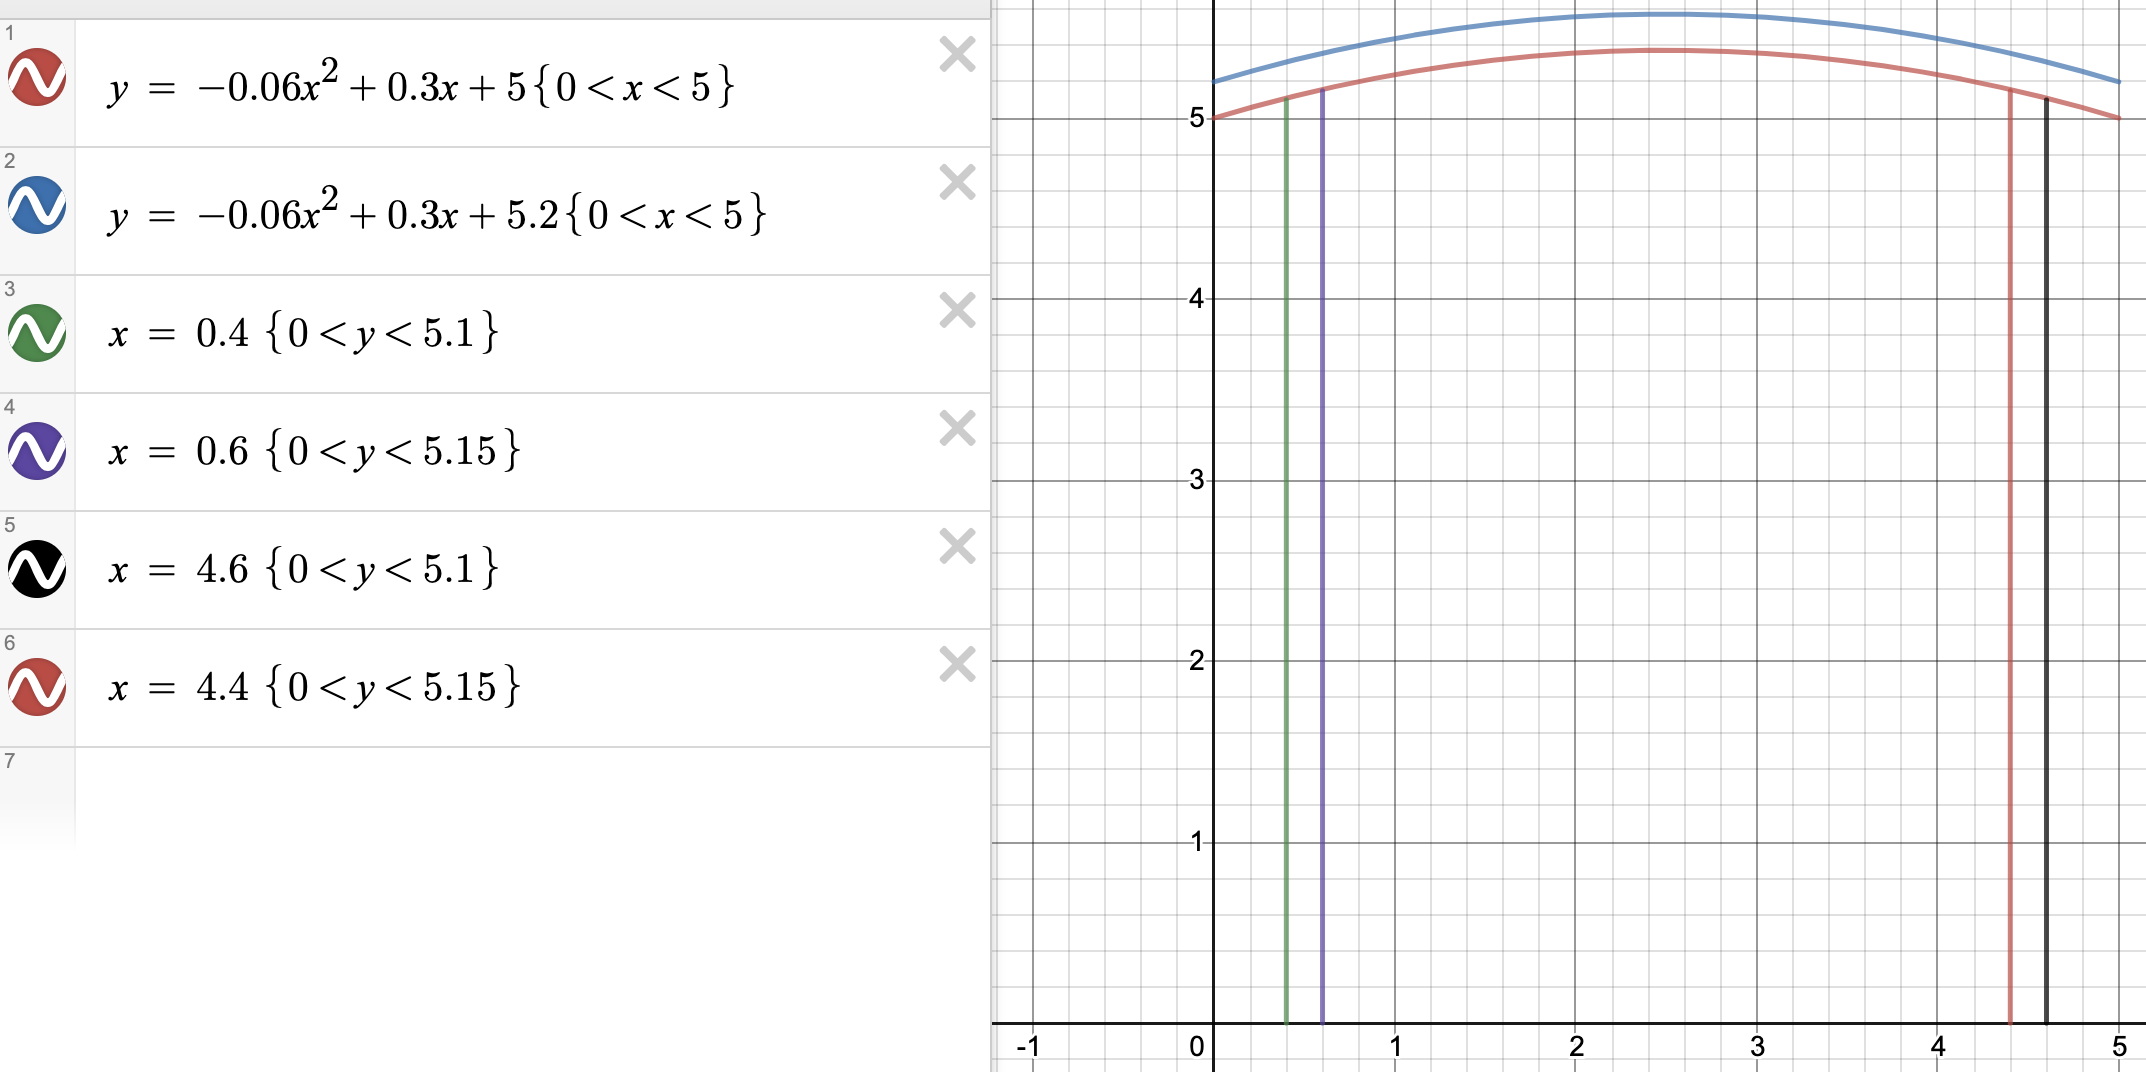
\includegraphics[width=\textwidth]{zhiBingDesign.png}
    \caption{Graph of Zhi Bing's final design}
    \label{fig:zhiBingDesign}
\end{figure}

\begin{align}
    f(x)&=-0.06x^2+0.3x+5
\end{align}

\subsubsection{Sunlight Heat dispersion}

\begin{figure}[htbp]
    \centering
    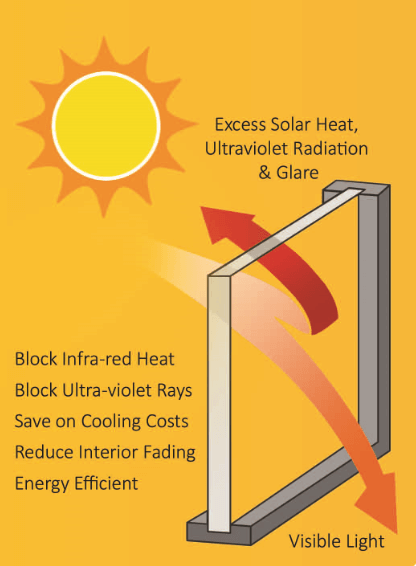
\includegraphics[width=7cm]{heatGlass.png}
    \caption{Simple visualisation of how the glass could work}
    \label{fig:heatGlass}
\end{figure}

Due to the downward concave shape of the sheltered walkway, it could cause a lot of light to be focused into the underside of the sheltered walkway. This causes it to heat up substantially, especially in the afternoon when most students are dismissed from school. A possible solution could be to use a special kind of glass for the roof that mitigates this. This material, developed by scientists at The Agency for Science, Technology and Research (A*STAR) \cite{sciencedaily-heat}, as seen in Figure \ref{fig:heatGlass}, ``blocks 90 per cent of the heat from sunlight'', letting only the sunlight light through. 

\pagebreak

\subsection{Weighing Designs}\label{sec:Other Feasible Models:Weighing Designs}

\subsubsection{Characteristics}

\begin{enumerate}
    \item Compare and contrast the different designs from your team members and decide on the best possible design based on the team’s data analysis, research and assumptions.
    \item What are some of the factors and variables the team considered in designing a covered walkway?
    \item How does the team simplify the problem using mathematical modelling?
    \item What are some of the assumptions and calculations involved in the design chosen?
\end{enumerate}

This table was a much simplified representation of the discussions the 4 of us have held in order to choose the best design.

\begin{table}[htbp]
    \centering
    \small
    \setlength\tabcolsep{2pt}
    \begin{tabular}{l|l|l}
        Design & Pros & Cons \\
        \hline
        \multirow{3}{4em}{Ryan} & Blocks Rain effectively  & Long and large, uses more materials \\& More factors considered &\\& Calculated different materials' viability &\\& Unique design &\\
        \hline
        \multirow{2}{4em}{Elliot} & Fits in with SST's aesthetic and & Will not be able to block out as much\\ & Is easier for construction & rain compared to a quadratic\\
        \hline
        \multirow{2}{4em}{Xavier} & Quadratic, so it is able to block out more rain & Weird shape\\  & Allows sunlight to pass through so there \\ &  is natural lighting &\\
        \hline
        Zhi Bing & Reflect sunlight + Blocks rain & Many assumptions, may be unrealistic \\
    \end{tabular}
    \caption{Table weighing pros and cons of various plausible designs by the team}
    \label{tab:prosAndConsOfDifferentDesigns}
\end{table}

\subsubsection{Weighing Pros vs Cons}

With the pros and cons stated above, the data can be tabulated into a checklist to determine which design fulfills the most factors.

\begin{table}[htbp]
\begin{tabular}{l|c|c|c|c}
\textbf{Factor} & \textbf{Ryan} & \textbf{Elliot} & \textbf{Xavier} & \textbf{Zhi Bing} \\
\hline
Blocks rain effectively & \checkmark &  & \checkmark & \checkmark \\
Fits with SST aesthetics & \checkmark & \checkmark & \checkmark  &  \\
Most factors considered & \checkmark &  &  &  \\
Diverts rain water from shelter & \checkmark & & \checkmark &  \\
Prevents collection of water & \checkmark & \checkmark & \checkmark & \checkmark \\
Considered materials used & \checkmark &  &  &  \\
Reflects sunlight & \checkmark &  &  & \checkmark 
\end{tabular}
\end{table}

In conclusion, since Ryan's design fulfills the most factors, it is the most optimal, based on the checklist created.

\pagebreak
\section{Conclusion}\label{sec:Conclusion}

\subsection{Optimal Design}\label{sec:Conclusion:Optimal Design}

In conclusion, the most optimal solution for the walkway shelter between SST's school gate to the general office, would be a shelter which long-side cross-section is modelled by a quadratic function,  $y=\left(-\frac{25}{1892}\right)x^{2}-\frac{303}{10}\left(-\frac{25}{1892}\right)x+2.5$, and short-side cross-section modelled by a quartic function, $y=-0.1x^4+0.6x^3-1.125x^2+0.675x$, made of a PVC plastic cover, supported by Steel columns, with a hexagonal tessellation frame, as seen in Figure \ref{fig:finalLongSide} and \ref{fig:finalShortSide}.

\begin{figure}[htbp]
    \centering
    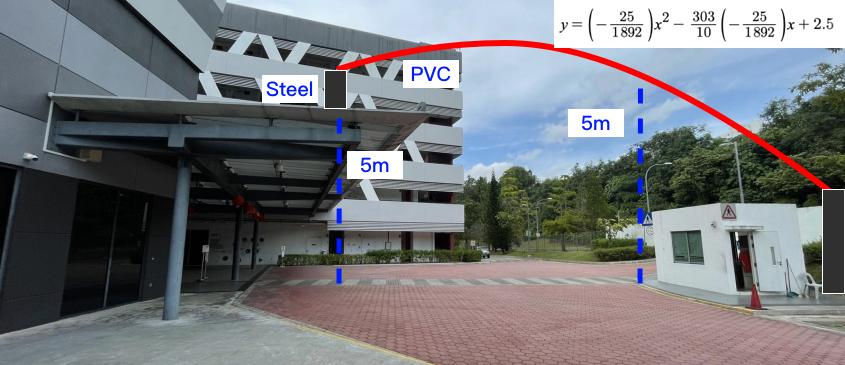
\includegraphics[width=\textwidth]{finalLongSide.png}
    \caption{Final proposal based on the various mathematical models from long-side viewpoint}
    \label{fig:finalLongSide}
\end{figure}

\begin{figure}[htbp]
    \centering
    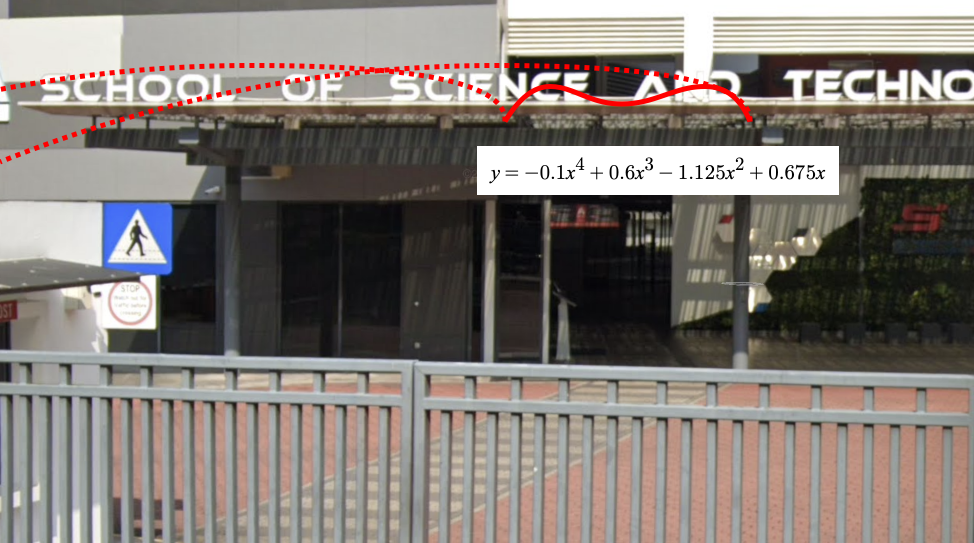
\includegraphics[width=\textwidth]{finalShortSide.png}
    \caption{Final proposal based on the various mathematical models from short-side viewpoint}
    \label{fig:finalShortSide}
\end{figure}

\pagebreak
\bibliographystyle{plain}
\bibliography{references}
\end{document}
